\chapter{Construction of the Brownian Motion [Professor Toaldo]}
\section{Lecture 1}
\subsection{Overview}
We are going to deepen the analysis part of this topic with Professor Badiale. \\
Now, imagine we want to describe a random phenomenon, so we deal with a random process:
\begin{equation*}
    \begin{split}
        &(X_t)_{t \geq 0} =: X\\
        &t \mapsto X_t (\omega) \quad \text{map from index set to state space}
    \end{split}
\end{equation*}
Now, the variation is 
\begin{equation*}
    dX_t = X_{t+dt} - X_t 
\end{equation*}
Notice that we are talking heuristically, not rigorously. \\
Now, let us assume that the variation is proportional to the time variation through a constant depending on the current position $c(X_t)$. What we obtain is a differential equation, together with the initial condition:
\begin{equation*}
    \begin{split}
        & d X_t= c(X_t) dt  \\
        & X_0=x
    \end{split}
\end{equation*}
The thing is that this equation is not random, since it is deterministic once we know $dt$ and the constant. We can therefore add a noise $(Y_t)$, thus obtaining a random differential equation:
\begin{equation}
\label{eq 1}
    dX_t = c(X_t) dt + \sigma Y_t
\end{equation}
The noise can be seen as 
\begin{equation*}
    Y_t \approx \sum_{k=1}^n \frac{Z_k}{n}
\end{equation*}
Letting $n$ go to infinity, by the central limit theorem, the noise is distributed as a Gaussian random variable:
\begin{equation*}
    Y_t \stackrel{CLT}{\approx} \mathcal{N}(0,dt)
\end{equation*}
The main idea is that we are summing up a countable number of elements which constitute a very small noise, scantly affecting the entire process. Nevertheless, their entirety in sum affects the process, representing the main noise. \\     
We may want to make the noise independent of $t$ yet dependent on the time lag $dt$. 

%the variance has a precise meaning,  so we set it like above.

So now, remember that the increments of the Brownian Motion are normally distributed:
\begin{equation*}
    B_{t+dt}-B_t \sim \mathcal{N}(0,dt)
\end{equation*}
With this in mind, we can rewrite \eqref{eq 1} as 
\begin{equation*}
    dX_t = \underbrace{c(X_t) dt}_{\text{deterministic}}  + \underbrace{\sigma(X_t) dB_t}_{\text{random}}
\end{equation*}
where we are also considering $\sigma$ not constant anymore, but instead depending on the current position $X_t$.\\
Now we have an heuristic point of view of the course but mathematically we still need to define some elements to have an idea of what we are talking about. 
\begin{equation}
\label{def eq}
    dX_t = c(X_t) dt + \sigma(X_t) dB_t
\end{equation}
An additional aim is to make $c(X_t)$ and $\sigma(X_t)$ dependent on time too, namely $c_t(X_t)$ and $\sigma_t(X_t)$. \\
We try to interpret \eqref{def eq} as a classical differential equation by taking derivatives:
\begin{equation*}
    \frac{d}{dt} X_t = c(X_t) + \sigma(X_t) \frac{d}{dt}B_t
\end{equation*}
The problem is that we know that "The Brownian motion is nowhere differentiable" so this interpretation is not good mathematically. \\
Then we try with the integral form:
\begin{equation*}
    X_t- X_0 = \int_0^t c(X_t) ds + \underbrace{\int_0^t \sigma(X_t) dB_s}_{\text{Itô integral}}
\end{equation*}
which is more promising since the BM is continuous and it is reasonable to think that we can integrate it. \\
The main point here is that the Riemann integral is not sufficient, since it does not work for all $\sigma$. If we want to extend the possible choice of $\sigma$ we need another construction for the integral and this leads to the theory of \textbf{Itô integration}. We recall the notion of \textbf{Riemann-Stieltjes integral}, which basically replaces the increments $\Delta s_i$ of the Riemann integral with the ones relative to a function $g$:
\begin{equation*}
    \int_0^t f_s dg_s := \lim_{n \to \infty} \sum_{i=1}^n f(\xi_i) \Delta g(s_i)
\end{equation*}
The problem is that when $g$ is a stochastic process, the integral could not converge. That's why we need a very regular process and a new definition of integral to deal with Brownian Motion. \\
So to sum up we need 
\begin{itemize}
    \item Notion of solution
    \item Existence and Uniqueness of it
\end{itemize}
To better clarify the role of the factors $c(X_t)$ and $\sigma(X_t)$, we make use of parabolic partial differential equations, of which an example is hereby reported:
\begin{equation}
\label{equation_L}
    \frac{\partial}{\partial t} q(x,t)= L q(x,t) \hspace{0.5 cm} q(x,0)=u(x)
\end{equation}
with $x \in \mR$, where $L$ is an operator given by 
\begin{equation*}
    L= a(x)\frac{\partial}{\partial x}  + b(x) \frac{\partial^2}{\partial x^2}
\end{equation*}
In the general case, $L$ could be added some other factors (like integrals).\\
A particular case is the heat equation in which analytical methods work perfectly
\begin{equation*}
    \frac{\partial}{\partial t} q(x,t)= \frac{\partial^2}{\partial x^2} q(x,t) 
\end{equation*}
In particular, the result is given by 
\begin{equation*}
    q(x,t) = \mathbb{E}^x[u(X_t)]
\end{equation*}
from which we get 
\begin{equation*}
    dX_t=b(X_t) dt + \sigma(X_t)dB_t
\end{equation*}
$b(X_t)$ corresponds to $a(x)$, while $\sigma(X_t)$ is relative to $b(x)$. \\
So, using probability we can approach partial differential equations and get methods to solve them. \\
Now, for difficult PDE's neither analytical nor numerical methods help to solve it. For example, the following provides an approximation converging to the solution of \eqref{equation_L}
\begin{equation*}
    q(x,t) \approx \frac{1}{N} \sum_{k = 1}^N u(X_t^k)
\end{equation*}
This is the scenario for Monte Carlo method, through which we can approximate it. \\
Recalling the equation we determined above, 
\begin{equation*}
    dX_t = b(X_t) dt + \sigma(X_t)dB_t
\end{equation*}
since the randomness comes from $\sigma(X_t)dB_t$, we need to know whether the Brownian Motion exists or not. This will be the goal of this chapter, but first let us recall some definitions and notions. 
\vspace{2 cm}
\section*{Revision}
\begin{DefBox}
    \begin{Def}
    $(E, \mathcal{E})$ and $(F, \mathcal{F})$ two measurable spaces, then 
    \begin{equation*}
        \begin{split}
        E \times F = \{(x,y): x \in E, y \in F\}\\
        A \subset E, B \subset F \quad A \times B = \{(x,y): x \in A, y \in B\}   \\    
        \mathcal{E}\otimes  \mathcal{F} = \sigma(\text{measurable rectangles})\\
        A \in \mathcal{E}, B\in \mathcal{F} \quad A\times B  \quad \text{ measurable rectangle}
        \end{split}     
    \end{equation*}
\end{Def}
\end{DefBox}
This isn't enough for stochastic processes since we need an infinite version:
\begin{DefBox}
    \begin{Def}
    $T$ arbitrary set ( $T=[0, \infty)$ ). For each $t \in T$, consider $(E_t, \mathcal{E}_t)$ a measurable space, $x_t \in E_t$ for each $t\in T$, $x:=(x_t)_{t \in T}$ is a function on $T$. \\
    $T \owns t \mapsto x_t \in E_t$ (where usually $E_t \equiv E \quad \forall t \in T$ for stochastic processes).\\
    $F:=\{\text{set of all such functions  } x = (x_t)\}$ is the \textbf{product space}.
\end{Def}
\end{DefBox}

\begin{DefBox}
    \begin{Def}
    A measurable rectangle in $F$ is a subset of $F$
    \begin{equation*}
        \bigtimes_{t \in T} A_t =\{x \in F: x_t\in A_t \quad \forall t \in T\}
    \end{equation*}
    where $A_t$ differs from $E$ ($E_t$) only for a finite number of $t \in T$.
\end{Def}
\end{DefBox}
Then a rectangle is measurable if $A_t \in \mathcal{E}_t$ for every $t \in T$, and the product sigma algebra is the one generated by all measurable rectangles:
\begin{equation*}
    \otimes_{t \in T} \mathcal{E}_t =\sigma \{\text{measurable rectangles}\}
\end{equation*}
\paragraph{Example} \begin{equation*}
    \begin{split}
        &E=\mR \hspace{1 cm} T=[0,\infty)\\
        &(\mR^{[0, \infty)}, \mathcal{B}^{[0, \infty)})
    \end{split}
\end{equation*}
The Borel-sigma algebra is countably measurable since it is generated by countably many measurable rectangles. It is a countable union of functions with \emph{finite} fixed positions. 
\begin{PropBox}
    \begin{Proposition}
    Let $(\Omega, \mathcal{A})$ be a measurable space and let $(F,\mathcal{F}) = \bigtimes _{t \in T} (E_t, \mathcal{E}_t)$. For each $t\in T$ let $f_t: \Omega \to E_t$. For each $\omega \in \Omega$ define $f(\omega)$ to be the point $(f_t(\omega))_{t \in T}$ in F. \\
    Then $f: \Omega \to F$ is $\mathcal{A}$-measurable (on $(A, \mathcal{F})$) $\iff$ $f_t$ is $\mathcal{A}$-measurable for every $t \in T$ (on $(A, \mathcal{E}_t)$).
\end{Proposition}
\end{PropBox}
Hence, we can characterize the measurability of a function on the product space based on the measurability of its components on a single set $E_t$ for every $t \in T$. 
\subsection{Brownian Motion}
Let $(\Omega, \mathcal{A}, \mathbb{P})$ be a probability space. 
\begin{DefBox}
    \begin{Def}
    A $d$-dimensional stochastic process $(B_t)_{t \geq 0} = : B$ on $(\Omega, \mathcal{A}, \mathbb{P})$ is a Brownian Motion if:
    \begin{itemize}
        \item $B_0 = 0$ almost surely 
        \item independent increments: $B_{t_i} - B_{t_{i-1}} \coprod$ for $i = 1, \ldots, n \quad n \in \mathbb{N}, t_0 < \ldots < t_n$
        \item stationary increments: $0 \leq s \leq t: B_t - B_s \sim B_{t-s}$
        \item Gaussian increments: $B_t - B_s \sim \mathcal{N}(0, (t-s) \mathbbm{1})$
        \item the trajectories $t \mapsto B_t(\omega)$ are continuous $\forall \omega \in \Omega$. 
    \end{itemize}
\end{Def}
\end{DefBox}
We will see that the course is greatly centered around the probability space $(C_0, \mathcal{B}_{C_0}, \mathbb{P})$ called Wiener space, where $C_0$ is the set of continuous functions, $\mathcal{B}_{C_0}$ is the Borel sigma-algebra and $\mathbb{P}$ is the Wiener measure.

\newpage

\section{Lecture 2}
We wrote the equation \eqref{def eq} whose solution is $X_t$ and in particular we said that the term $\sigma(X_t) dB_t$ adds randomness. The problem is that we need to be sure about the existence of the Brownian Motion to write and treat such an equation. Now, we are going to construct it. \\  
Actually, to construct and prove the existence of the BM there are two approaches:
\begin{itemize}
    \item the \textbf{Lévy construction}, which only works for the Brownian Motion
    \item the \textbf{canonical construction}, which is used for many processes and consists in fixing a probability space $(C_0(I)), \ldots, \ldots)$ with $C_0(I)$ space of continuous functions, then identifying a $\sigma$-algebra and a probability measure to obtain a BM. To do so, we use $X(\omega) = \omega$ as a process.
\end{itemize}
We want to find a probability space $(\Omega, \mathcal{F}, \mP)$ and a r.v. on it satisfying the definition. The Kolmogorov Theorem allows to do it. Recall first that we are going to work with 
\begin{equation*}
    \mathbb{R}^I = \{\omega: I \to \mathbb{R}\} = \bigtimes _{t \in I} \mathbb{R}, \quad \mathcal{B}^I(\mathbb{R}) = \bigtimes_{t \in I} \quad \text{ product $\sigma$-algebra }
 \mathcal{B}(\mathbb{R})
 \end{equation*}
 considering therefore the space $(\mathbb{R}^I, \mathcal{B}^I(\mathbb{R}))$.
\begin{ThBox}
    \begin{Th}[Kolmogorov Theorem]
    For each $t_1, \dots, t_n \geq 0$ and for every $n \in \mathbb{N}, $ with $t_j \neq t_k$, $j \neq k$, let $p_{t_1, \dots, t_n}(\cdot, \dots, \cdot)$ be a probability measure on $(\mR^n, \mathcal{B}(\mR^n))$ (for fixed times $t_i$). \\
    Assume that this family satisfies the so-called consistency conditions:
    \begin{enumerate}
        \item $p_{t_1, \dots, t_n}(A_1 \times  \dots \times  A_n) = p_{t_{\sigma(1)}, \dots, t_{\sigma(n)}}(A_{\sigma(1)} \times  \dots \times  A_{\sigma(n)})$ where $\sigma:\{1, \dots, n\} \to \{1, \dots, n\} $ is a permutation of $\{1, \ldots, n\}$;
        \item $p_{t_1, \dots, t_{n-1}}(A_1\times  \dots \times  A_{n-1}) =p_{t_1, \dots, t_{n-1}, t_n}(A_1\times  \dots \times  A_{n-1}\times \mR) $
    \end{enumerate}
    Then there exists a (unique) probability measure $\mu$ on the product space $(\mR^{[0,\infty)}, \mathcal{B}^{[0,\infty)}(\mR))$ such that the canonical process $X=(X_t)_{t \geq 0}$ with $X_t(\omega)= \omega(t)$ has finite dimensional distribution 
    \begin{equation*}
        \mP(X_{t_1}\in A_1, \dots, X_{t_n} \in A_n)= p_{t_1, \dots, t_n}(A_1 \times \dots \times  A_n)
    \end{equation*}
    for any $t_1, \dots, t_n$, $n \in \mathbb{N}$.
\end{Th}
\end{ThBox}

\begin{PropBox}
    \begin{Cor}
    There exists a unique measure $\mu$ on $(\mR^I,\mathcal{B}^I(\mR) )$ such that the canonical process $X=(X_t)_{t \geq 0}$ satisfies $X_0=0$ almost surely, has  stationary and independent increments. 
\end{Cor}
\end{PropBox}
\begin{ProofBox}
\begin{proof}[Sketch of the proof]
    Let $p_{t_1, \dots, t_n}$ be Gaussian $(\underline{0}, C)$, $C_{ij}= min(t_i, t_j)$. The Gaussian distribution satisfies the consistency conditions. 
\end{proof}
\end{ProofBox}
Now, the next thing we need is the continuity of trajectories. Define
\begin{equation*}
    C_0=\{\omega \in \mathbb{R}^I \text{s.t. } \omega \text{ is continuous and } \omega(0) = 0\}
\end{equation*}
We would like to have $\mu(C_0) = 1$, but we are not sure about its validity. The problem is that the product $\sigma$-algebra is too small and the Kolmogorov theorem holds on the product $\sigma$-algebra.
\begin{PropBox}
    \begin{Lemma}
    For every $I \in \mathcal{B}^I(\mathbb{R})$ there exists on at most countable set $S \subset [0,+\infty)$ s.t. $v \in I, \omega \in \mathbb{R}^I, v|_S = \omega |_S$, then $\omega \in I$. 
\end{Lemma}
\end{PropBox}
Therefore, $C_0 \notin \mathcal{B}^{[0,+\infty)}$. So, not all the elements contain continuous functions and hence we cannot compute the probability $\mu(C_0)$. The solution to this problem is provided by the following theorem.
\begin{ThBox}
    \begin{Th}[Kolmogorov-Centsov]
    Let \((X_t)_{t \geq 0}\) be a \(d\)-dimensional process in \((\Omega, \mathcal{F}, \mathbb{P})\). If there are constants \(c > 0\), \(\alpha > 0\), and \(\beta > 0\) such that:
    \begin{equation*}
        \mathbb{E} \left( |X_t - X_s|^\alpha \right) \leq c |t - s|^{1 + \beta}, \quad \text{for all } s, t \geq 0
    \end{equation*}
then \(X_t\) has a version with exclusively only continuous trajectories.
\end{Th}
\end{ThBox}
Recall that a version of a process is a process itself $(Y_t)_{t \geq 0}$ such that 
\begin{equation*}
    \mathbb{P}(X_t = Y_t) = 1 \quad \text{ for all } t \geq 0
\end{equation*}
\begin{equation*}
    \begin{split}
        & (\mathbb{R}^{[0, +\infty)}, \mathcal{B}^{[0,+\infty)}(\mathbb{R}), \mu) \quad X \rightarrow Y \\
        & Y: \mathbb{R}^{[0,+\infty)} \hookrightarrow C_0 \\
        & (C_0, \mathcal{B}(C_0), \mathbb{P})
    \end{split}
\end{equation*}
If we put together these two results we get the continuity of trajectories! \\
Take $(\mathbb{R}^I, \mathcal{B}^I(\mathbb{R}), \mu)$ and use $Y=(Y_t)_{t \in I}$ which is the Kolmogorov-Centsov version of the canonical process on $(\mathbb{R}^I, \mathcal{B}^I(\mathbb{R}))$. Then, take $(C_0(I), \mathcal{B}(C_0(I)), P)$ where $P$ is the Wiener measure and $B = (B_t)_{t \geq 0}$ is the canonical process on $(C_0(I), \mathcal{B}(C_0(I)), P)$. 

\chapter{Properties of the Brownian Motion [Professor Toaldo]}
In this chapter we want to deepen the main known results about the oscillation of the Brownian Motion, whose trajectories are pretty irregular in time. \\
In particular, the basic notions to keep in mind are the following
\begin{itemize}
    \item $t \mapsto B_t(\omega)$ is continuous 
    \item almost surely, $t \mapsto B_t(\omega)$ has no points where it is differentiable
    \item $t \mapsto B_t(\omega)$ has no bounded variation almost surely on any finite interval $[a,b]$, that is the vertical distance run by the BM in finite time from $a$ to $b$ is always infinity
    \item almost surely, the BM has no monotone interval, that is the probability that there exists an interval such that the BM is monotone inside equals $0$. 
\end{itemize}
Consider a continuous function $f:[0,+\infty) \rightarrow \mathbb{R}$ and suppose we want to know the distance run by $f$ on $[0,t]$, that is the oscillation over this interval. The latter should be given approximately by $f(t) - f(0)$, which can be roughly approximated in turn by the sum of oscillations of $f$ over small consecutive intervals $[t_0, t_1] \ldots [t_{n-1}, t_n]$ with $0 = t_0 \leq \ldots \leq t_n = t$. 
\begin{equation*}
    |f(t_1) - f(t_0)|+|f(t_2) - f(t_1)|+ \ldots
\end{equation*}
We could try to improve the quality of the approximation by letting the amplitude of the intervals go to $0$. 
\begin{DefBox}
    \begin{Def}[strong $p$-variation]
    Let $f:[0,+\infty) \to \mathbb{R}$ be a function on $\Pi := \{0 = t_0 < t_1 < \ldots < t_n = t\}$, a partition of $[0,t]$ with mesh $|\Pi| := \max_j |t_j - t_{j-1}|$. For $p > 0$ we call 
    \begin{align*}
        S_p^\Pi(f,t) &= \sum_{t_j \in \Pi} |f(t_j) - f(t_{j-1})|^p\\
        &= \sum_{j=1}^n |f(t_j) - f(t_{j-1})|^p
    \end{align*}
    is the p-variation sum of $f$ along $\Pi$. \\
    We call $\text{VAR}_p(f,t) := \sup\{S_p^\Pi(f,t): \Pi \text{ partition of } [0,t]\}$ the strong (or total) $p$-variation.
\end{Def}
\end{DefBox}

\begin{remark}
    If $\text{VAR}_1(f,t) < \infty$, then $f$ is of bounded variation.  
\end{remark}

\begin{DefBox}
    \begin{Def}[$p$-variation]
    Let \( f \colon [0, \infty) \to \mathbb{R} \) and let \( (\Pi_n)_{n \in \mathbb{N}} \) be a sequence of partitions of \([0, t]\) with \( |\Pi_n| \to 0 \) as \( n \to \infty \). 

Then, the \(p\)-variation of \(f\) over \([0,t]\) is defined as:

\[
\text{Var}_p(f, t) := \lim_{n \to \infty} S_p^{\Pi_n}(f, t)
\]

where \( S_{\Pi_n}(f, t) \) denotes the sum associated with the partition \(\Pi_n\).
\end{Def}
\end{DefBox}
We want $f$ to be the Brownian Motion path, depending on the trajectories:
\begin{equation*}
        f_t \equiv B_t(\omega)   
\end{equation*}
This means that we should clarify in which sense the limit which defines the p-variation exists. That's, in particular, because $(\Pi_n)_{n \in \mathbb{N}}$ are typically not allowed to depend on $\omega$.       \\
The main result is the following.
\begin{ThBox}
    \begin{Th}[Quadratic variation of BM]
    Let $(B_t)_{t \geq 0}$ be a one-dimensional Brownian Motion. Let $(\Pi_n)_{n \in \mathbb{N}}$ be a sequence of partitions of $[0,t]$ s.t. $|\Pi_n| \rightarrow 0$. Then
    \begin{equation*}
        VAR_2(B,t) := L^2-\lim_{n \rightarrow +\infty} S_2^{\Pi_n}(B,t) = t
    \end{equation*}
\end{Th}
\end{ThBox}
This means that the quadratic variation of the Brownian Motion equals $t$ in the $L^2$ sense. \\
Before providing the proof of the theorem, we remark that
\begin{remark}
    The sequence $\Pi_n$ is not allowed to depend on $\omega \in \Omega$. It is indeed possible to prove that for almost every $\omega \in \Omega$ there exists a sequence of partitions $(\Pi_n(\omega))_{n \in \mathbb{N}}$ of $[0,t]$ with $|\Pi_n(\omega)|\rightarrow 0$ such that
    \begin{equation*}
        \lim_{n \rightarrow \infty} S_2^{\Pi_n(\omega)}(B(\cdot, \omega), t) = \infty \quad \text{ a.s. }
    \end{equation*}
    Moreover, this implies also that VAR$_2(B(\cdot, \omega), t) = \infty$ almost surely. 
\end{remark}
\begin{ProofBox}
    \begin{proof}
    The thesis is 
    \begin{equation*}
        \lim_{|\Pi| \rightarrow 0} \mathbb{E}|S_2^\Pi(B,t) - t|^2 = 0
    \end{equation*}
    which is the $L^2$ norm. \\
    Let a partition $\Pi = \{0 = t_0 < t_1 < \ldots < t_n = t\}$ of $[0,t]$ be fixed and notice that
    \begin{equation*}
        \mathbb{E}(S_2^\Pi(B,t)) = \sum_{j=1}^n \mathbb{E}(B{t_j} - B_{t_j-t_{j-1}})^2 = \sum_{j=1}^n(t_j-t_{j-1}) = t
    \end{equation*}
    Then, by the independence of the increments and $\sum_{j=1}^n(t_j-t_{j-1}) = t$:
    \begin{align*}
        \mathbb{E}(S_2^\Pi(B,t)-t)^2 &= \mathbb{V}ar(S_2^\Pi(B,t)) \\
        &= \sum_{j=1}^{n} \mathbb{E} [(B_{t_j} - B_{t_{j-1}})^2 - (t_j - t_{j-1})]^2 \\
        &= \sum_{j=1}^{n} \mathbb{E} [B^2_{t_j - t_{j-1}} - (t_j - t_{j-1})]^2 \quad \text{by stationarity of the increments}\\
        &= \sum_{j=1}^{n} (t_j - t_{j-1})^2 \mathbb{E} [B_1^2 - 1]^2 \quad \text{since $B_t \stackrel{\text{d}}=\sqrt{t} B_1$}\\
        &\leq c \sum_{j=1}^{n} (t_j - t_{j-1}) (t_j - t_{j-1}) \\
        & \leq c \underbrace{|\Pi| }_{\text{ bound with maximum }} \sum_{j=1}^{n} |t_j - t_{j-1}| = c |\Pi| t \rightarrow 0 \quad |\Pi| \rightarrow 0
    \end{align*}
\end{proof}
\end{ProofBox}
\section*{Some other notions}
Since the $L^2$-convergence implies the existence of an almost surely convergent subsequence, the previous result also proves that there exists a subsequence $\Pi_{n_k}$ such that $S_2^{\Pi_{n_k}}(B,t) \rightarrow t$ almost surely. 
\begin{PropBox}
    \begin{Proposition}
    \begin{equation*}
        S_2^{\Pi_n}(B,t) \xrightarrow{L^2} t
    \end{equation*}
    There exists $(\Pi_{n_k})_{k \in \mathbb{N}}$ s.t. $S_2^{\Pi_{n_k}} (B,t) \xrightarrow{ \text{ a.s. }} t$.
\end{Proposition}
\end{PropBox}
We wonder how to find such subsequence and the answer is given by the following theorem.  
\begin{ThBox}
    \begin{Th}
    Let $(\Pi_n)_{n \in \mathbb{N}}$ be a sequence of partitions of $[0,t]$ with 
        \begin{equation}
        \label{assumption}
            \sum_n |\Pi_n| < +\infty
        \end{equation}
    Then, then $S_2^{\Pi_n}(B,t) \xrightarrow{ \text{a.s.}} t, n \rightarrow \infty$.
\end{Th}
\end{ThBox}
\begin{remark}
    The assumption \ref{assumption} implies that $|\Pi_n| \rightarrow 0$ sufficiently fast.
\end{remark}
\begin{PropBox}
    \begin{Proposition}
    \begin{equation*}
        VAR_p(B,t) = +\infty \text{  a.s. } \forall t \geq 0, p \leq 2
    \end{equation*}
\end{Proposition}
\end{PropBox}
For $p=2$ it is possible to find $\Pi_n(\omega)$ s.t. $\lim_{n\rightarrow +\infty} S_2^{\Pi_n(\omega)} (B,t) = +\infty$.\\
The idea is that if we consider the distance $|b-a| > 0$ of only one trajectory we get a very bad approximation, while if instead we take all the trajectories in average we obtain a pretty good approximation in  $L^2$. 
\begin{equation*}
    \int_0^t f dg := \lim_{|\Pi| \rightarrow 0} \sum_{t_j \in \Pi} f(\xi_j)(g(t_j) - g(t_{j-1}))
\end{equation*}
with $\xi_j \in [t_{j-1}, t_j)$. If we transform it into an $L^2$ integral adding the dependence on $\omega$, then the integral now converges. This is not the true definition of Itô integral though, of which we will give an easier approach later.
\chapter{(Ir)regularity of Brownian paths [Professor Toaldo]}
\begin{DefBox}
    \begin{Def}
    A function $f:[0,+\infty) \rightarrow \mathbb{R}$ is said to be locally Holder continuous of order $\alpha \in (0,1]$ if, for every $T>0$, there is a constant $c(T)$ s.t.
    \begin{equation*}
        |f(t)-f(s)| \leq c|t-s|^\alpha \quad s,t \in [0,T]
    \end{equation*}
\end{Def}
\end{DefBox}
The function is globally Holder continuous if $c(T) = c$ does not depend on T. 
\begin{ThBox}
    \begin{Th}
    Almost all Brownian paths are nowhere locally Holder-continuous for $\alpha>\frac{1}{2}$.
\end{Th}
\end{ThBox}
\begin{ProofBox}
    \begin{proof}
    Fix $\alpha > \frac{1}{2}$. Take $I=[a,b]$. Define 
    \begin{equation*}
        \mathcal{N}_{a,b} := \{\omega \in \Omega: \exists c(\omega) \text{  s.t.  } |B(t,\omega) - B(s,\omega)| \leq c(\omega) |t-s|^\alpha \quad \forall s,t \in [a,b]\}
    \end{equation*}
    We want to prove
    \begin{equation*}
        \mathbb{P}(\cup_{a,b} \mathcal{N}_{a,b}) = 0
    \end{equation*}
    Since $a,b \in [0,+\infty)$ they can be rationals, making the union countable. Therefore, since
    \begin{equation*}
        \mathbb{P}(\cup_{a,b} \mathcal{N}_{a,b}) \leq \sum_{a,b \in \mathbb{Q}}\mathbb{P}(\mathcal{N}_{a,b})
    \end{equation*}
    we need to prove $\mathbb{P}(\mathcal{N}_{a,b})=0$. Fix $\omega \in \mathcal{N}_{a,b}$ and suppose by contradiction the function is Holder continuous of order $\alpha$. 
    \begin{align*}
        S_2^{\Pi_n}(B(\cdot,\omega), [a,b]) &= \sum_{j=1}^n (B_{t_j}(\omega) - B_{t_{j-1}}(\omega))^2\\
        &\stackrel{\omega \in \mathcal{N}_{a,b}}\leq c^2(\omega) \sum_{j=1}^n |t_j - t_{j-1}|^{2\alpha+1-1} \\
        &\leq c^2(\omega) |\Pi|^{2\alpha -1} \sum_{j=1}^n|t_j-t_{j-1}| \rightarrow 0, \quad |\Pi| \rightarrow 0 
    \end{align*}
    We recall that 
    \begin{equation*}
        \sum_{j=1}^n|t_j-t_{j-1}| = b-a
    \end{equation*}
    On the other hand, since there exists a sequence of partitions $(\Pi_n)_{n \in \mathbb{N}}$ of $[a,b]$ with 
    \begin{equation*}
        |\Pi| \rightarrow 0 \quad \text{such that} \quad S_2^{\Pi_n}(B, [a,b]) \rightarrow b-a \text{   a.s. }
    \end{equation*}
    Therefore, since it is an arbitrary partition, it follows that $\mathbb{P}(\mathcal{N}_{a,b})=0$. \\
    This leads to a contradiction and to the proof of the thesis. 
\end{proof}
\end{ProofBox}

\newpage

\section{Lecture 3}
Last time we talked about the Wiener space $(\Omega, \mathcal{A}, \mP)$, in which we considered $B_t$ a Brownian Motion. Then, we defined the p-variation of the BM.\\
Now, we are going to keep discussing about the \emph{(ir)regularity} of the BM: in particular, we concluded that if we consider just one trajectory of the BM we do not achieve regularity, while instead if we consider the entirety of them we get it together with the convergence. \\
Keep in mind the result we stated last lecture about the almost sure Holder continuity of the trajectories: the BM paths are nowhere locally Holder continuous when $\alpha > \frac{1}{2}$, which is actually valid for $\alpha = \frac{1}{2}$ too (proof too difficult).\\
Let us now state a weaker version of the Kolmogorov-Centsov theorem. 
\begin{ThBox}
    \begin{Th}
    Let $(Y_t)_{t \geq 0}$ be a random process on $\mR$ with continuous paths. Let $T>0$. If there exists finite constants $c>0$, $\beta, \gamma >0$ s.t.
    \begin{equation*}
        \mE|X_t-X_s|^\gamma \leq c|t-s|^{1+\beta} \hspace{1 cm } s, t \in [0,T]    \end{equation*}
 Then, the paths $[0,T] \owns t \mapsto X_t (\omega)$ are a.s. Holder continuous of order $\alpha \in (0, \frac{\beta}{\gamma})$ and  
 \begin{equation*}
     \mE \Big[\sup_{0 < |s-t|< 1 \ \ s,t \in [0,T]} \frac{|X_t-X_s|}{|t-s|}\Big]^\gamma< \infty \hspace{ 1 cm} \alpha \in (0, \frac{\beta}{\gamma})
 \end{equation*}
\end{Th}
\end{ThBox}
\begin{PropBox}
    \begin{Cor}
    The paths $t \mapsto B_t(\omega)$ of the BM are a.s. locally Holder continuous for $\alpha < \frac{1}{2}$
\end{Cor}
\end{PropBox}
\begin{ProofBox}
    \begin{proof}
    \begin{equation*}
    \begin{split}
    \mathbb{E}[|B_t - B_s|^n] &\stackrel{ \text{stationarity}} = \mathbb{E}[|B_{t-s}|^n] \stackrel{ \text{scaling}} = |t-s|^\frac{n}{2} \underbrace{\mathbb{E}|B_1|}_{C \text{ const.}}\\
        \mE |B_t -B_s|^\gamma &\leq c |t-s|^{1+\beta}\\
        \text{ where }\gamma= n &\hspace{0.5 cm} \beta=  \frac{n}{2}-1\\
        \alpha < \frac{\beta}{\gamma}&= \frac{1}{2}-\frac{1}{n} \hspace{1 cm}
    \end{split}      
    \end{equation*}
    and for $n$ big enough we are able to reach the desired result.
\end{proof}
\end{ProofBox}
\begin{PropBox}
    \begin{Proposition}
\label{prop 1}
    For each fixed $T > 0$, then the Brownian paths $t \mapsto B_t(\omega)$ are not differentiable at $t=T$ almost surely. 
\end{Proposition}
\end{PropBox}
The strongest version of this concept that we can achieve is the following 
\begin{PropBox}
    \begin{Proposition}
\label{prop 2}
    The sample paths $t \mapsto B_t(\omega)$ are almost surely nowhere differentiable. 
\end{Proposition}
\end{PropBox}
The proof of \eqref{prop 1} comes from Stochastic Processes course, while the one of \eqref{prop 2} is in Toaldo's notes. \footnote{page $60$-$61$ file notes from last year}

A graphic representation is provided in Figure \ref{fig_1}. 

\begin{figure}
    \begin{center}
    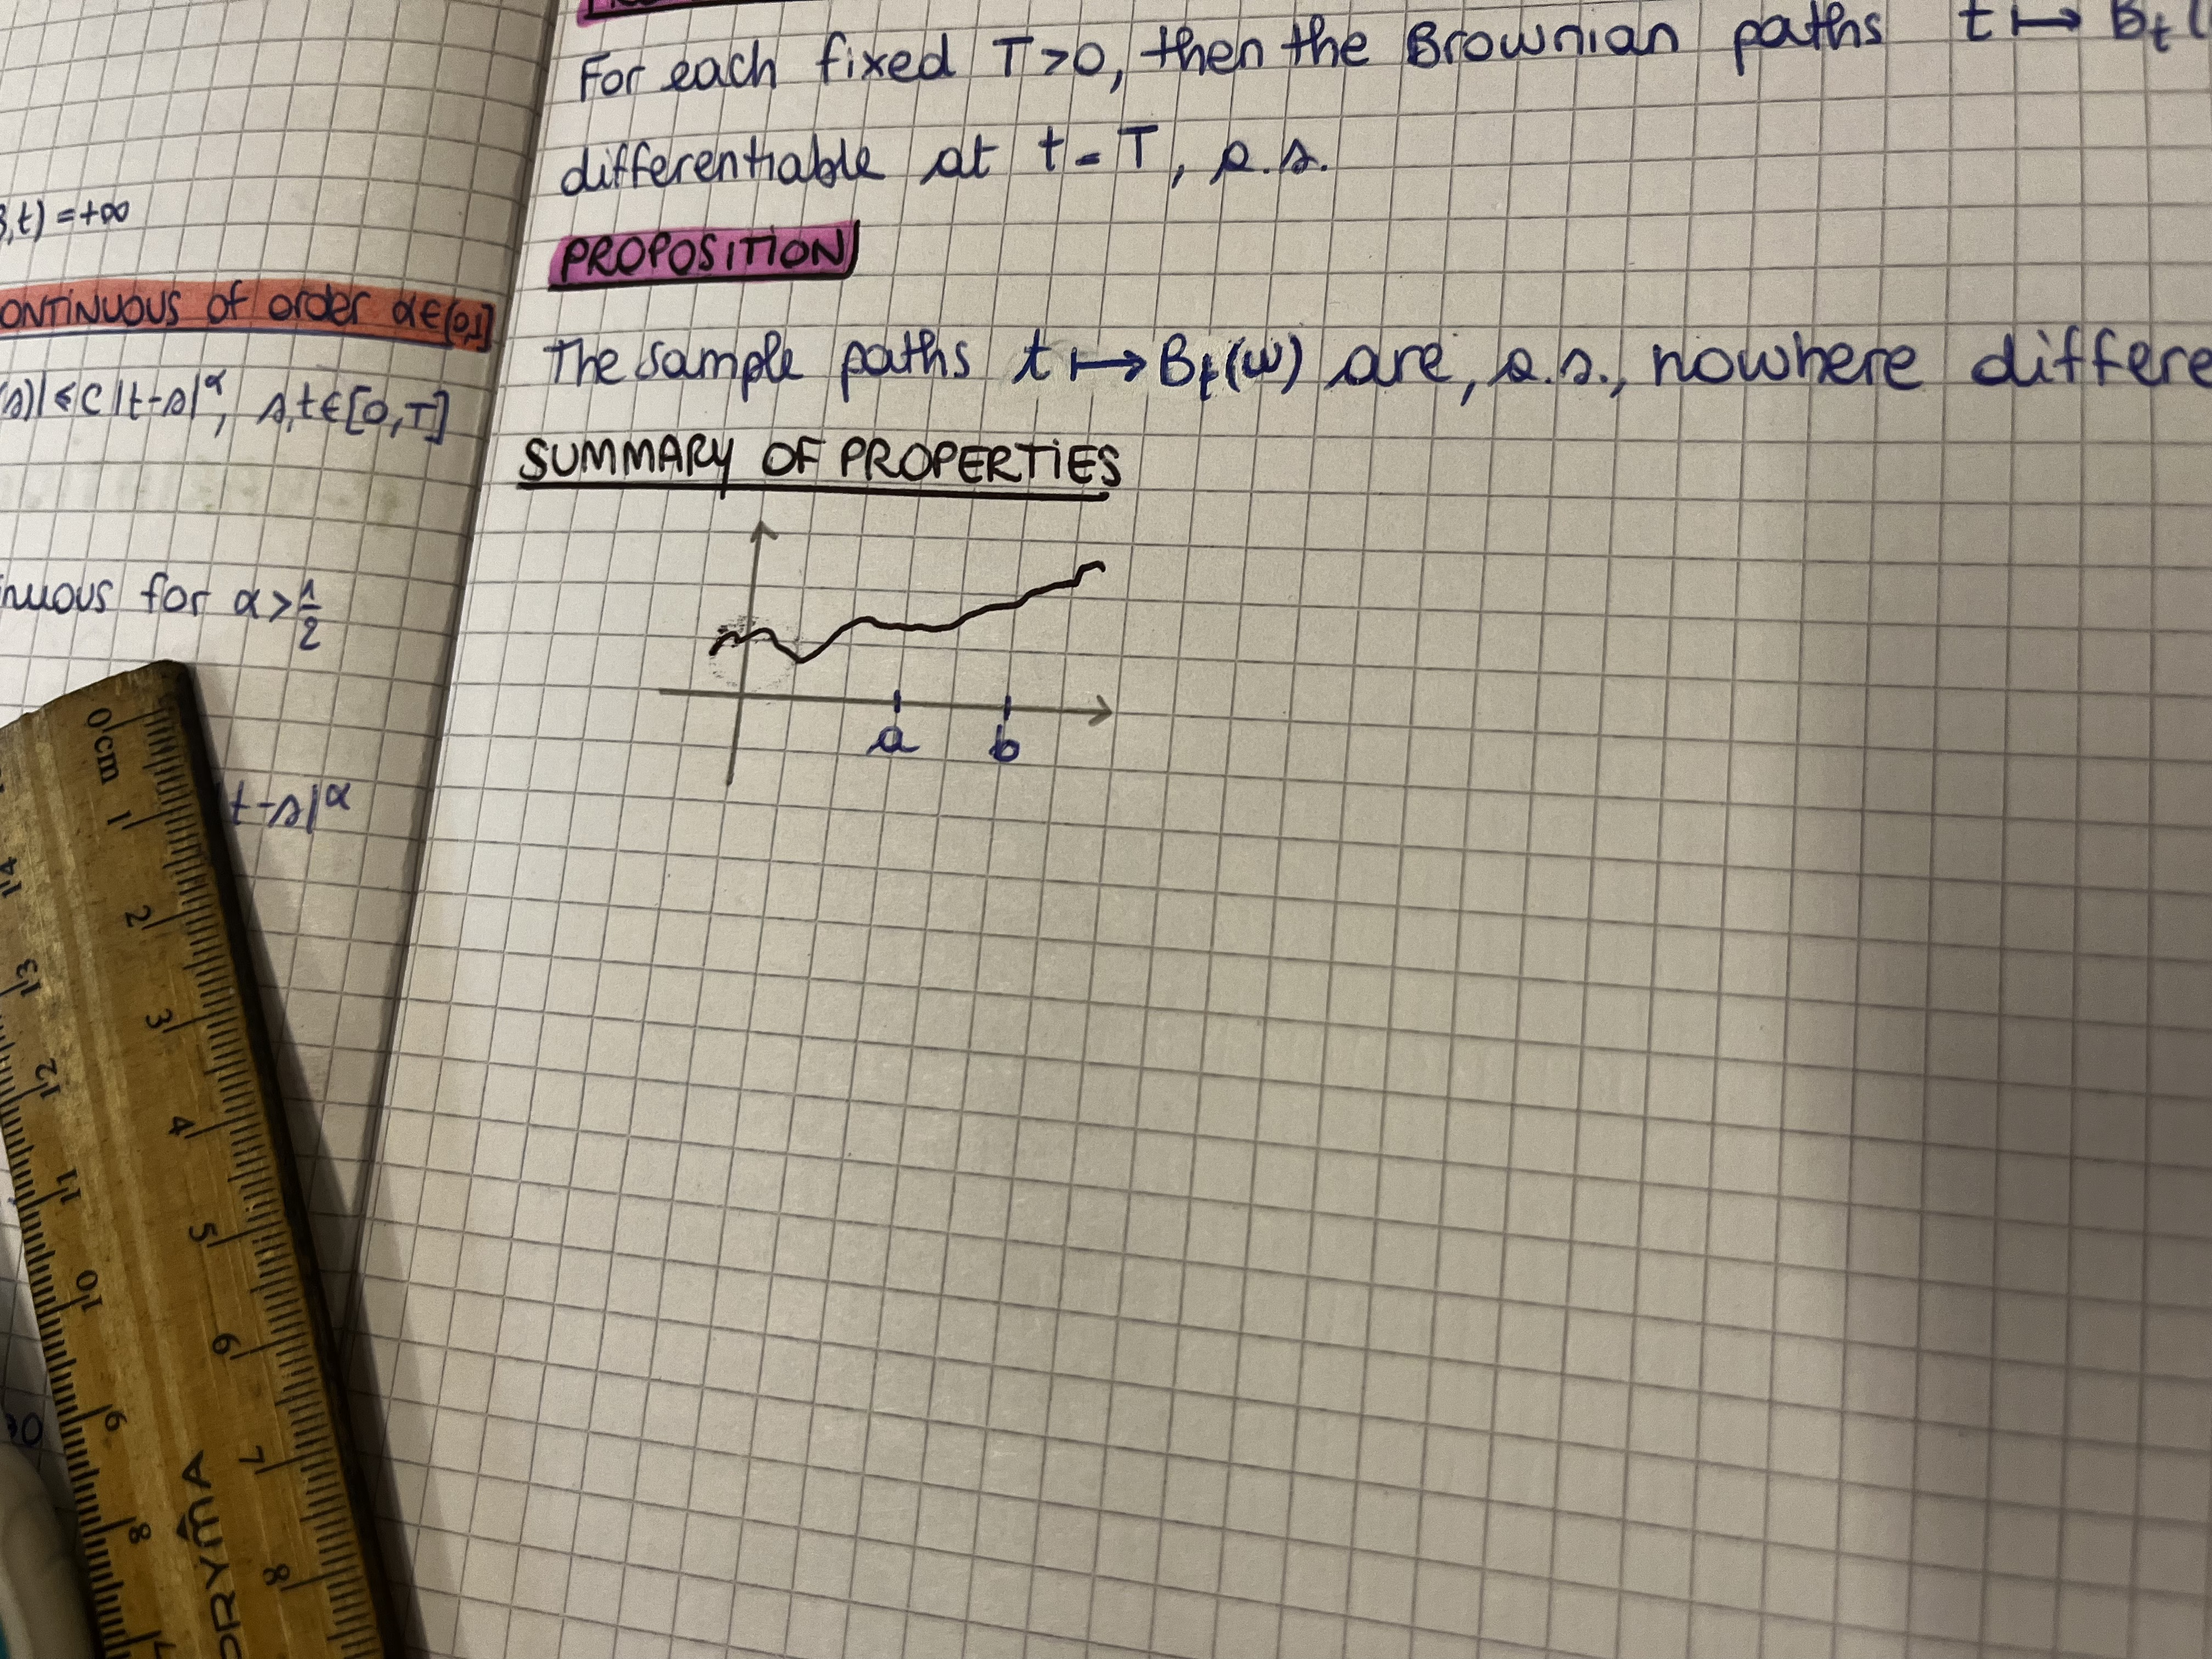
\includegraphics[width=14cm]{IMG_9589.jpeg}\\ 
    \caption{Non-differentiability of the BM} 
    \label{fig_1}
    \end{center} 
\end{figure} 

\begin{remark}
    In Stochastic Processes course we achieved this result by means of the following steps:
    \begin{itemize}
        \item Differentiability of a function in a point implies that the function itself is Holder continuous of order $\alpha = 1$ in a neighbourhood of the point.
        \item We proved, as above, that the path of a BM is \emph{not} Holder continuous of order $\alpha \geq \frac{1}{2}$ almost surely.
        \item Then, since the Holder continuity does not hold for $\alpha \geq \frac{1}{2}$, it cannot be valid in particular for $\alpha = 1$. Therefore, by the result in the first item, we get that the function (that is, the BM path) is nowhere differentiable. 
    \end{itemize}
\end{remark}
\begin{PropBox}
    \begin{Proposition}
    With probability $1$, there is no interval $[a,b] \subset (0,+\infty)$ where $t \mapsto B_t$ is monotone. 
\end{Proposition}
\end{PropBox}
\begin{remark}
    This is true also in $\mathbb{R}^d$. 
\end{remark}
Regardless of the length of the interval $[a,b]$ we consider, provided that it is finite, we will never find either monotone increasing or monotone decreasing paths. Instead, they will always be oscillating. \\
Moreover, even if the interval we pick has very small length, the distance ran by the
function will always be infinite. Indeed, from Stochastic Processes course, we know that the oscillations of the BM are infinite and of small amplitude. \\
The goal of the lecture is to show that the following approach does not work.
\begin{equation*}
\begin{split}
    d X_t &= b_c(X_t) dt + \sigma_t(X_t)dB_t\\
    X_t -X_0 &= \int_0^t b_s(X_s) ds + \int_0^t \sigma_s(X_s)dB_s\\
    \int_0^t &\sigma_s(X_s(\omega))dB_s(\omega)
\end{split}
\end{equation*}

\chapter{Stochastic Integration [Professor Toaldo]}
First of all, we recall the main concepts of the \emph{Riemann integration}, which is our starting point. \\
Consider an interval $I=[a,b]$ and imagine we want to integrate a function $f: [a,b] \to \mathbb{R}$ on this interval. Then we consider a partition of the interval 
\begin{equation*}
\begin{split}
     \Pi_n &:= \{a = x_0 < x_1 < \ldots < x_n = b\}\\
    \sum_{j=0}^{n-1} &f(\xi_j) (x_{j+1} - x_j) \quad \xi_j \in [x_j, x_{j+1}]
\end{split}
\end{equation*}

If the limit of the previous sum exists and it equals a constant $C$, then when the mesh of the partition decreases to $0$
\begin{equation*}
    |\Pi_n| \rightarrow 0 
\end{equation*}
\begin{equation}
    \int_a^b f(t) dt:= c
\end{equation}
\begin{remark}
    According to the Riemann integration, for $\int_a^b f(t) dt$ to exist, the function must be \textbf{continuous}, that is $f \in \mathcal{C}([a,b])$. This is a \emph{sufficient} condition. 
\end{remark}
If we are interested in the integration of a function against the increments of another one, we extend the Riemann integral to the \emph{Riemann-Stieltjes} integral:
\begin{equation*}
    \int_a^b f(t)dg(t)
\end{equation*}
We take the sum
\begin{equation*}
    \sum_{j=0}^{n-1} f(\xi_j)(g(x_{j+1})-g(x_j)) \hspace{1 cm} \xi_j \in [x_j, x_{j+1}]
\end{equation*}
letting the mesh of the partition go to $0$
\begin{equation*}
    |\Pi_n|\ra 0
\end{equation*}
The two conditions for the Stieltjes integral of $f$ to exist are:
\begin{itemize}
    \item $f$ and $g$ without any discontinuity at the same point $x$ $\rightarrow$ \emph{necessary} condition.
    \item $f$ is continuous and $g$ is of bounded variation, $\rightarrow$ \emph{sufficient}, but \emph{not} necessary condition.
\end{itemize}
\begin{equation}
    \int_0^t \sigma_s(X_s) dB_s \stackrel{Riemann-Stieltjes} = ?
\end{equation}
We are not sure that this integral actually exists. 

If we want to use the notion of integral to integrate along the trajectory we need this integral to cover at least all the continuous functions. Therefore, it's reasonable to require that the integral we are defining 
exists for any $f \in \mathcal{C}([0,T])$.
\begin{equation*}
    \int_0^T f(s) dB_s
\end{equation*}
The problem is given by the following result 
\begin{PropBox}
    \begin{Proposition}
    Let $\alpha:[a,b]\to \mR$ and denote 
    \begin{equation*}
        I(f):= \int_a^bf(t)d\alpha(t)
    \end{equation*}
    If this integral exists as a Riemann-Stieltjes integral for all $f \in \mathcal{C}([a,b])$, then $\alpha$ is of bounded variation, that is:
    \begin{equation*}
    ||\alpha||_{TV} = \sup_{\Pi} \sum_{t_i \in \Pi} |\alpha(t_i)-\alpha(t_{i-1})| < + \infty
\end{equation*}
\end{Proposition}
\end{PropBox}
If we want to use RS integral as a notion to integrate BM, then this is basically hopeless. That's because if we want the integral to cover all the continuous functions over compact intervals, the function must be of bounded variation. The problem is that BM \emph{is not} of bounded variation and so we cannot apply this notion of integral. Therefore, we must define a new kind of integration object to be able to integrate the BM. \\
The Riemann-Stieltjes integral exists, but not for all the continuous functions. \\
For example, the sum does not converge considering the following integral:
\begin{equation*}
    \int_0^t B_s dB_s
\end{equation*}
What's the solution? We must consider all the trajectories of the BM. 
    \begin{PropBox}
        \begin{remark}
        \textbf{Banach-Steinhaus.} Let $(X, ||\cdot||_X)$ and $(Y, ||\cdot||_Y)$ be Banach spaces and let $I$ be any index set. For each $i\in I$, let $S_i: X \to Y$ be a continuous linear map. If 
        \begin{equation*}
            \sup_{i \in I} ||S_i(x)||_Y < \infty \hspace{1 cm} x \in X
        \end{equation*}
    then 
    \begin{equation*}
         \sup_{i \in I} \underbrace{ \sup_{||x||_X \leq 1} ||S_i(x)||_Y < \infty }_{\text{operator norm}}
    \end{equation*}
    \end{remark}
    \end{PropBox}
    We are now going to use this theorem to prove the previous proposition. 
    \begin{proof}
    Consider 
    \begin{itemize}
        \item $X = \mathcal{C}([a,b]), \quad || \cdot || _{\infty}$ as norm 
        \item $Y = \mathbb{R}$
        \item $I$: family of all finite partitions of $[a,b]$, $\Pi = \{a = t_0 < \ldots < t_n = b\}, n \in \mathbb{N}$. 
    \end{itemize}
    Now, let $\Pi \in I$ and define
    \begin{equation*}
       S_\Pi(f) := \sum_{i=1}^n f(t_i) (\alpha(t_i)-\alpha(t_{i-1})) \hspace{0,5 cm} f \in C[a,b]
    \end{equation*}
    Fixing any partition, it is clear that $f \mapsto S_\Pi(f)$ is a linear map. We can therefore apply Banach - Steinhaus theorem:
    \begin{align*}
        |S_\Pi(f)| &\stackrel{(*)}\leq ||f||_{\infty} \sum_{i=1}^n |\alpha(t_i)-\alpha(t_{i-1})| \\ 
        &= C_{\Pi, \alpha} ||f||_{\infty}
    \end{align*}
    where $(*)$ is given by the fact that $f$ is bounded, being continuous over a compact interval. \\
    Therefore, $S_\Pi$ is a bounded (hence continuous) linear map.\\
    Since 
    \begin{equation}
    \label{condition}
        S_\Pi(f) \rightarrow \int_a^b f(t) d\alpha(t) \quad \forall f \in \mathcal{C}([a,b])
    \end{equation}
    as $|\Pi| \rightarrow 0$, then 
    \begin{equation*}
       \sup_\Pi |S_\Pi(f)| < + \infty
    \end{equation*}
    Indeed, if by contradiction the supremum was infinite, then it would be so over a set of partitions with mesh going to $0$. Nevertheless, we will never reach infinity because of the assumption about convergence in \eqref{condition}.\\
    Therefore, by Banach-Steinhaus,
    \begin{equation*}
        \sup_\Pi \sup_{||f||_\infty \leq 1} |S_\Pi(f)|<+ \infty
    \end{equation*}
    Now, we want to use this to prove that the function $\alpha$ must be of bounded variation, that is 
    \begin{equation*}
        ||\alpha||_{TV} < +\infty
    \end{equation*}
    This is true since
    \begin{equation*}
    \begin{split}
        ||\alpha||_{TV} &= \sup_\Pi \sum_{i=1}^n |\alpha(t_i)- \alpha(t_{i-1})|\\
        &= \sup_\Pi S_\Pi(f_\Pi)\\
        & \stackrel{(*)}\leq \sup_\Pi \sup_{||f||_\infty \leq 1} |S_\Pi(f)| < \infty
    \end{split}
    \end{equation*}
     \begin{figure}
\begin{center} 
  % Requires \usepackage{graphicx} 
  \includegraphics[width=14cm]{IMG_9591.jpeg}\\ 
  \caption{$f$ piecewise linear}
  \label{fig_2}
\end{center} 
\end{figure} 
    The last inequality $(*)$ is justified as follows. We consider $f$ piecewise linear (as in Figure \ref{fig_2}) with
    \begin{align*}
        f_\Pi(t_i) &= \text{sign}(\alpha(t_i) - \alpha(t_{i-1}))\\
        & \stackrel{ \text{R.S.}}\leq \sup_{\Pi} \sup_{||f||_{\infty} \leq 1} |S_\Pi(f)| < +\infty
    \end{align*} 
\end{proof}
\begin{remark}
    In practice, what we understand is that - since the Brownian paths are almost surely not of bounded variation - they cannot be defined as a RS integral $\int_0^T f(t) dB_t$ if the class of admissible integrands contains all continuous functions $f$ on $[0,T]$.
\end{remark}
To solve the problem, we change the kind of convergence.  
\chapter{Ito Integral [Professor Toaldo]}
\begin{equation*}
    \lim_{|\Pi| \ra 0} \sum_{t_i \in \Pi}f(t_i) (B(t_{i+1})-B(t_i))
    \end{equation*}
could be infinite for $f \in \mathcal{C}([a,b])$. In practice, the idea is to modify the convergence considering the $L^2$ limit $L^2 - \lim_{|\Pi| \rightarrow 0}$: we do not consider the BM path by path, but we consider instead the entirety of the trajectories. We are now giving a definition of Lebesgue integral, to move finally on to the Ito integral.
\begin{DefBox}
    \begin{Def}
    Consider a \textbf{positive simple function} $f$, that is 
    \begin{equation*}
        f = \sum a_i \mathbbm{1}_{[t_{i-1}, t_i)}
    \end{equation*}
and its \textbf{integral} over the interval $[a,b]$:
    \begin{equation*}
        \int_a^b f(t)dt=\sum_{i_1}^n a_i|t_i -t_{i-1}| \hspace{2 cm} t_i \in \Pi
    \end{equation*}
    We know that, for every positive simple function (piecewise constant), there exists a sequence of functions $f_n \uparrow f$. Therefore
    \begin{equation*}
        \int_a^b f dt  = \lim_{n \rightarrow +\infty}\int_a^b f_n dt
    \end{equation*}
    Considering the decomposition involving positive and negative parts of the function
    \begin{equation*}
        f = f^+ - f^-
    \end{equation*}
    we get 
    \begin{equation*}
        \int_a^b f dt = \int_a^b f^+ dt - \int_a^b f^- dt 
    \end{equation*}
\end{Def}
\end{DefBox}
We divide the interval $[a,b]$ into $n$ sub-intervals and look at approximating sums
\begin{equation*}
    S_n = \sum_{j = 1}^n f(B_{s_j}) (B_{t_{j+1}} - B_{t_j}) \quad s_j \in [t_j, t_{j+1}]
\end{equation*}
Since the variation of the BM paths is not bounded, the pointwise limit of $S_n$ does not exist and therefore we cannot use RS definition of integral. \\
However, we are going to see that if we consider $S_n$ as an element of $L^2(\Omega, dP)$, then it \emph{does} have a limit. \\
Unfortunately, even in this setting, the limit will depend on how the point $s_j$ is chosen, unlike the RS case. \\
For this first part of the discussion, we will restrict on $s_j = t_j$, meaning that we will choose the integrand to be adapted to the filtration. 

\begin{DefBox}
    \begin{Def}[Step process]
    Let $[S,T] \subset \mR$ be an interval and let $(\mathcal{F}_t^B)_{t \geq 0}$ be the natural filtration of BM. We call $(f_t)_{t \in [S,T]}$ a \textbf{random step process} if there is a partition $S=t_0 < t_1 < \dots < t_n =T$ and random variables $\eta_0, \eta_1, \ldots, \eta_{n-1} \in L^2(\Omega, dP)$ such that $\eta_j$ are $\mathcal{F}_{t_j}^B$-adapted and 
    \begin{equation*}
        f_t = \sum_{j=0}^ {n-1} \eta_j \mathbbm{1}_{[t_j, t_{j+1}]}(t)
    \end{equation*}
    meaning that $f_t$ is a simple function. 
\end{Def}
\end{DefBox}
\begin{DefBox}
    \begin{Def}
    We denote by 
    \begin{equation*}
        M^2_{\text{step}}([S,T])
    \end{equation*}
    the class of random step processes.
\end{Def}
\end{DefBox}
\begin{remark}
    In general, a step process is not a Markov process.
\end{remark}
\begin{DefBox}
    \begin{Def}
    Let $f_t \in M^2_{\text{step}} ([S,T])$. We define the \textbf{Ito integral of $f_t$} with respect to the BM by
    \begin{align*}
        I(f)&:=: \int_S^T f_t dB_t \\
       &:= \sum_{j=0}^{n-1} \eta_j (B_{t_j} - B_{t_{j-1}})
    \end{align*}
\end{Def}
\end{DefBox}
The two definitions are equivalent and the latter one shows the similarity to the Lebesgue integral definition.  \\
We remark that the integral is a random variable, not a number, since it depends on $\omega$. 
\begin{PropBox}
    \begin{Proposition}
    For every $f_t \in  M^2_{\text{step}}([S,T]) $ we have 
    \begin{equation*}
        I(f) \in L^2(\Omega, dP)
    \end{equation*}
    that is, $I(f)$ is a random variable in $L^2$.
    Moreover, the $L^2$-norm is:
    \begin{equation*}
        \underbrace{\mathbb{E}[I(f)]^2}_{||I(f)||^2_{L^2(\omega)}} = \underbrace{\mathbb{E}[\int_S^T f_t^2 dt]}_{||f||^2_{L^2(\Omega \times [S,T])}} \quad \text{ called \textbf{Ito isometry}}
    \end{equation*}
    It is called isometry since it is an equality between the norms on two different spaces: the first one concerns a random variable on $\Omega$, while the second one is on $\Omega \times [S,T]$. 
\end{Proposition}
\end{PropBox}
\begin{remark}
    This is true for general processes too.
\end{remark}
\begin{ProofBox}
    \begin{proof}
Denote 
    \begin{equation*}
        \Delta_jB = B_{t_{j+1}} - B_{t_j} \quad \text{ and }  \quad \Delta_j t= t_{j+1} - t_j
    \end{equation*}
    Then,
    \begin{align*}
        [I(f)]^2 &= \Big[\sum_{j=0}^{n-1} \eta_j (B_{t_{j+1}} - B_{t_j})\Big]^2 \\
        &= \sum_{j=0}^{n-1}\sum_{k=0}^{n-1}\eta_j\eta_k \Delta_j B\Delta_k B    \\
        &= \sum_{j=0}^{n-1} \eta_j^2 (\Delta_j B)^2 + 2 \sum_{k>j} \eta_j\eta_k \Delta_j B\Delta_k B 
    \end{align*}
    Now, consider $j < k$ and compute (using Tower Rule and independence of increments)
    \begin{align*}
        \mE [\eta_j \eta_k \Delta_j B \Delta_k B] & \hspace{0 cm } \stackrel{ \text{tower rule}}{=} \mathbb{E} \mathbb{E}[\eta_j \eta_k \Delta_j B \Delta_k B | \mathcal{F}_{t_k}^B] \\
    &\stackrel{\text{conditional determinism}}{=} \eta_j \Delta_j B \eta_k \underbrace{\mE[\Delta_k B| \mathcal{F}_{t_k}^B ]}_{\mathbb{E}[\Delta_k B] = 0} \\
    & \hspace{1,5 cm }= 0\\
    \end{align*}
Taking the expectation:
    \begin{align*}
    \mE[I(f)]^2 &= \mathbb{E}\Big[\sum_{j=0}^{n-1} \eta_j^2(\Delta_j B)^2\Big] +0 \\
    &= \sum_{j=0}^{n-1}\mE \eta_j^2 (\Delta_j B)^2\\
    &= \sum_{j=0}^{n-1}{\mE \underbrace{ \mE [\eta_j^2(\Delta_j B)^2 |\mathcal{F}_{t_j}^B]}_{\mE(\Delta_j B)^2= \Delta_j t}}
    \end{align*}
    since $ \eta_j \in L^2(\Omega, dP)$,  $\mE \eta_j < + \infty$ and so  $\mE [I(f)]^2 < + \infty$. Now, consider that 
    \begin{align*}
        f_t^2 &= \sum_{j = 0}^{n-1} \sum_{k=0}^{n-1} \eta_j \eta_k \mathbbm{1}_{[t_j,t_{j+1})}{(t)} \mathbbm{1}_{[t_k, t_{k+1})}{(t)}\\
        &= \sum_{j = 0}^{n-1} \eta_j^2 \mathbbm{1}_{[t_j, t_{j+1})}{(t)} 
    \end{align*}
    which means that 
    \begin{equation}
    \label{result}
        \mathbb{E}\int_S^T f(t)^2 dt = \sum_{j=0}^{n-1} \mathbb{E}\eta_j^2\Delta_j(t)
    \end{equation}
    Indeed: 
    \begin{equation*}
        \mE \int_S^T f_t^2 dt= \mE \int_S^T \sum_{j = 0}^{n-1} \eta_j^2 \mathbbm{1}_{[t_j, t_{j+1})}^{(t)} dt= \sum_{j = 0}^{n-1} \mE \eta_j^2 \Delta_j(t)
    \end{equation*}
    Using \ref{result} together with 
    \begin{equation*}
        \mathbb{E}I(f)^2 = \sum_{j=0}^{n-1} \mathbb{E}\eta_j^2 \Delta_j t
    \end{equation*}
    proved above we can conclude the proof.
\end{proof}

\end{ProofBox}
\section{Lecture 4}
To define the Ito integral with respect to BM for more general integrals, we are going to approximate integrands by random step processes. To this aim, we introduce the space of random processes as follows. 
\begin{DefBox}
    \begin{Def}
    $M^2(S,T)$ is the class of real valued stochastic processes 
    $f: \mR^+ \times \Omega \to \mR$ such that 
    \begin{itemize}
        \item $(t,\omega) \mapsto f_u(\omega)$ is measurable, for every $u \in [S,T]$ with respect to $([S,u] \times \Omega, \mathcal{B}([S,u]) \otimes \mathcal{F}_u^B)) \to (\mathbb{R}, \mathcal{B}(\mathbb{R}))$. This property is called \textbf{progressive measurability}. 
        \item $\mathbb{E}[\int_S^T f_t^2 dt]< +\infty$ that is, the $L^2$ norm must be finite. 
    \end{itemize}
\end{Def}
\end{DefBox}
What this definition tells us is that $f$ must be a function of the Brownian Motion, measurable with respect to its filtration with respect to $\omega$. The first condition concerns regularity with respect to the Borel $\sigma$-algebra and as a function of time. 

\begin{PropBox}
    \begin{Proposition}
\label{prop_progressive}
    Let $X$ be a right continuous process adapted to $\mathcal{F}_t^B$. Then it is progressively measurable.
\end{Proposition}
\end{PropBox}
\begin{remark}
    $M^2_{\text{ step}}$ is right continuous, therefore it is progressively measurable. 
\end{remark}
Consider the following \\
\textbf{Example} Imagine we want to integrate the process $X$, in particular:
\begin{equation*}
    Y_t = \int_0^t X_s ds \hspace{2 cm} X=(\Omega, \mathcal{F}, \mathcal{F}_t, X_t, \mP)
\end{equation*}
We want to make sure that this integral actually exists and is well-defined on $X$. 
In particular, we wonder whether the mapping $\omega \mapsto Y_t(\omega)$ is a random variable in $\mathcal{F}_t$ or not. \\
We know that if $X$ is progressively measurable, then the map 
\begin{equation}
\label{ex_map}
    (\omega, s) \mapsto X_s(\omega) 
\end{equation}
is $\mathcal{F}_t \otimes \mathcal{B}([0,t])$-measurable. By Fubini's theorem the map
\begin{equation*}
    \omega \mapsto \int_0^t X_s(\omega) ds 
\end{equation*}
is $\mathcal{F}_t$-measurable. It follows that $Y$ is adapted to $\mathcal{F}_t$ and also progressively measurable, since it is continuous. We report hereby the Fubini's theorem statement. 
\begin{ThBox}
    \begin{Th}[\textbf{Fubini's Theorem}]
    Let $\mu_1$ and $\mu_2$ be measures on $(E_1, \mathcal{E}_1)$ and $(E_2, \mathcal{E}_2)$ measurable spaces and $f: E_1 \times E_2 \to \mR$ measurable with respect to $\mathcal{E}_1 \otimes \mathcal{E}_2$. Suppose that at least one of the following is true 
    \begin{itemize}
        \item $f$ is integrable with respect to $\mu_1 \otimes \mu_2$
        \item $f$ is positive 
    \end{itemize}
    Then it is true that 
    \begin{itemize}
        \item the following functions are measurable with respect to $\mathcal{E}_1$ and $\mathcal{E}_2$ respectively. 
        \begin{equation*}
            \begin{split}
                x_1 \mapsto \int f(x_1,z) &\mu_2(dz) \hspace{2 cm} \in \mathcal{E}_1\\
                x_2 \mapsto \int f(z, x_2) &\mu_1(dz) \hspace{2 cm} \in \mathcal{E}_2
            \end{split}
        \end{equation*}
        \item \begin{align*}
            \int _{E_1 \times E_2} f d\mu_1 \otimes d\mu_2 &= \int \mu(dx_1) \int f(x_1, x_2) \mu(dx_2) \\
            &= \int \mu(dx_2) \int f(x_1, x_2) \mu(dx_1)
        \end{align*}
    \end{itemize}
\end{Th}
\end{ThBox}
Now, recall the equation we stated in the previous lectures:
\begin{equation*}
    dX_t = \underbrace{b_t(X_t) dt}_{\text{Riemann int}} + \underbrace{\sigma_t(X_t) dB_t }_{\text{Itô int}} 
\end{equation*}
A corollary of Proposition \ref{prop_progressive} is the following
\begin{Cor}
    $M^2_{\text{step}}([S,T]) \subset M^2([S,T])$ 
\end{Cor}
Indeed, $M^2_{\text{step}}$ processes are right continuous and therefore progressively measurable too. \\
In practice, we are enlarging the class of functions that can be integrated since the functions are not required to be step processes anymore. The usage of step processes is crucial since they are dense in $M^2$.

\begin{Lemma}
\label{lemma_2}
    Suppose $(f_t)_{t \in [S,T]} \in M^2(S,T)$. Then, there exists a sequence $(\phi^n)_{n \in \mathbb{N}} \subset M^2_{\text{step}}([S,T])$ such that 
    \begin{equation*}
        \mathbb{E}\big[\int_S^T |f_t(\omega) - \phi_t^ n(\omega)|^2 dt\big] \ra 0, \quad \text{for } n \ra +\infty
    \end{equation*}
\end{Lemma}
This can be written as 
\begin{equation*}
    \mathbb{E}[\int_S^T |f_t - \phi_t^ n|^2 dt] = ||f_t - \phi_t||_{L^2(\Omega \times [S,T])} \ra 0 \hspace{ 2 cm} n \ra + \infty
\end{equation*}


This lemma tells us that whenever we pick a random process that we want to integrate, then we can identify a class of $L^2$ step processes converging to it. It's the same as what happens with Lebesgue integral, in which there exists a sequence of positive functions converging to the integrated function. The difference here is that the sequence converges to the function $f$ not point-wise but in $L^2$.  

\begin{ProofBox}
    \begin{proof}[Sketch of the proof]
We prove roughly the statement proceeding in $4$ steps. \\
   \emph{Step 1}: consider $g_t \in M^2(S,T)$ bounded and such that $t \to g_t (\omega)$  is continuous, for every $\omega \in \Omega $.
   \begin{equation*}
   \Phi_t^n:= \sum_j g_{t_j}(\omega) \mathbbm{1}_{[t_j, t_{j+1})}{(t)}
   \end{equation*}
   \begin{equation*}
       L^2(\Omega \times [S,T])- \lim_{n \ra \infty} \phi_t^n = g_t 
   \end{equation*}
   In this step, we prove the Lemma under the hypothesis of \emph{bounded and continuous} functions. \\
   \emph{Step 2}: $h_t \in M^2(S,T)$ bounded. Let $\psi^n(s)$ non-negative, continuous and supported on $K \subset [-\frac{1}{n}, 0] $ and such that 
   \begin{equation*}
       \int \psi^n(s) = 1
   \end{equation*}
   Then
   \begin{equation*}
       g_t(\omega)= \int_0^t \psi^n(s_t) h_s(\omega) ds 
   \end{equation*}
   is continuous and bounded.
   \begin{equation*}
       L^2(\Omega \times [S,T])- \lim_{n \ra +\infty} g^n_t(\omega) = h_t
   \end{equation*}
   In this step we use Step $1$ implicitly to prove the entire Lemma whenever $h_t$ is \emph{only bounded} and not continuous. \\
   Step 3: Let $f \in M^2(S,T)$
   \begin{equation*}
   h_t^n(\omega) = 
       \begin{cases}
         - n & f_t(\omega) < -n \\
         f_t(\omega) & -n < f_t(\omega) < n\\
         n & f_t(\omega) > n
       \end{cases}
   \end{equation*}
   is bounded. 
   \begin{equation*}
       L^2(\Omega \times [S,T])-\lim_{n \rightarrow +\infty} h_t^n(\omega) = f_t
   \end{equation*}
   In this step we get rid of the hypothesis about boundedness too, to prove the entire Lemma for functions in $M^2$. \\
   Finally, by the previous steps, we conclude that we can always find a step process satisfying the statement. 
\end{proof}
\end{ProofBox}
Here, similarly of Lebesgue integration, we remove each time an assumption up to generality. This time, though, we work in the $L^2$ space. \\
Now, putting together the density of $M^2_{\text{step}}$ in $M^2$ and the Ito Isometry, what we get is the definition of Ito integral on $M^2$. \\
Recall that density means that whenever we pick a process in $L^2$ we can find a sequence of step processes converging to it. 
\begin{equation*}
    (\phi_t^n)_{n \in \mathbb{N}} \subset M^2_{\text{step}}, f_t \in M^2 \quad \text{such that} \quad \phi_t^n \rightarrow f_t \quad L^2(\Omega \times [S,T])
\end{equation*}
We know that we can define Ito integral for any $L^2$ step process \\

Now, the aim is to prove that the sequence of integrands is convergent in $L^2$ to a limit, which will be exactly the Ito integral. 
\begin{equation*}
    I(f):= L^2-\lim_n \int_S^T \phi_t^n dB_t
\end{equation*}
The best way to prove it is to show it is a Cauchy sequence. 
Immagine we want to define 
\[
I(f) := \lim_{n \to \infty} \int_S^T \phi_n(t) \, dB_t.
\]
We notice two problems with this definition: 
\begin{itemize}
    \item first of all we are not sure about the convergence of $\phi_n(t) \, dB_t$
    \item second of all, even if it converges, we have no certainty about the meaningfulness of this definition
\end{itemize}  
The answer to the second question is negative, in fact we need a definition of $L^2$-limit.\\
For the convergence problem we check that the previous Lemma combined with the Ito isometry implies that 
\begin{equation*}
    (\int_S^T \phi_t^n dB_t)_{n \in \mathbb{N}}
\end{equation*}
is a $L^2(\Omega)$ - Cauchy sequence. This way, $\int_S^T \phi_t^ndB_t$ must converge to a random variable in $L^2(\Omega)$ as $n \rightarrow +\infty$. \\
To prove it, we use the following 
\begin{Lemma}
    The Ito integral on $M^2_{\text{step}}$ is linear, that is 
    \begin{equation}
        I(\alpha_1 f^1+\alpha_2 f^2) = \alpha_1 I(f^1) + \alpha_2I(f^2)
    \end{equation}
\end{Lemma}
\begin{ProofBox}
    \begin{proof}
    Recall the definition of Ito integral of $f$ with respect to the BM:
    \begin{equation*}
        I(f) := \int_S^T f_t dB_t = \sum_{j=0}^{n-1} \eta_j (B_{t_j} - B_{t_{j-1}})
    \end{equation*}
    Then,
    \begin{align*}
         I(\alpha_1 f^1+\alpha_2 f^2) &=  \int_S^T (\alpha_1 f^1+\alpha_2 f^2) dB_t \\
         &= \int_S^T \alpha_1f^1 dB_t + \int_S^T \alpha_2 f^2 dB_t \\
         &= \alpha_1\int_S^T f^1 dB_t + \alpha_2\int_S^T f^2 dB_t \\
         &= \alpha_1 I(f^1) + \alpha_2I(f^2)
    \end{align*}
    by the linearity property of the integral. 
\end{proof}

\end{ProofBox}
Now we can prove that $(\int_S^T \phi_t^n dB_t)_{n \in \mathbb{N}}$ is in fact an $L^2(\Omega)$ - Cauchy sequence. 
\begin{ProofBox}
    \begin{proof}
We want to show that $\mE \big( \int_S^T \phi_t^n dB_t - \int_S^T \phi_t^m dB_t\big)^2 \xrightarrow{n,m \rightarrow + \infty} 0$.
\begin{align*}
        \mE \big( \int_S^T \phi_t^n dB_t - \int_S^T \phi_t^m dB_t\big)^2 &\stackrel{\text{linearity}}= \mE \big( \int_S^T (\phi_t^n - \phi_t^m) dB_t\big)^2 \\
        &\stackrel{\text{Ito isometry}} = \mathbb{E}\big( \int_S^T (\phi_t^n - \phi_t^m)^2 dB_t\big) \\
        &= || \phi_t^n - \phi_t^m ||_{L^2(\Omega \times [S,T], dt \times dt} \xrightarrow{n,m}0
\end{align*}
since by Lemma \ref{lemma_2}
\begin{equation*}
    ||\phi_t^n - f_t ||_{L^2(\Omega \times [S,T])}  \xrightarrow{n,m}0 
\end{equation*}
\end{proof}
\end{ProofBox}
\begin{DefBox}
    \begin{Def}
    Let $(f_t)_{t \in [S,T]} \in M^2 (S,T)$ and $(\phi^n)_{n \in \mathbb{N}} \subset M^2_{\text{step}}(S,T)$ such that 
    \begin{equation*}
        \phi^n \rightarrow f \quad \text{that is} \quad \lim_{n \rightarrow \infty} \mE\Big[\int_S^T |f_t - \phi_t^n | ^2 dt \Big] = 0
    \end{equation*}
     in $L^2(\Omega \times [S,T])$.\\
     Then, we define the \textbf{Ito integral of $(f_t)_{t \in [S,T]}$ on $[S,T]$} by
     \begin{align*}
         I(f) &:= \int_S^T f_t dB_t \\
         &:= L^2(\Omega)-\lim\int_S^T \phi^n_t dB_t
     \end{align*}
\end{Def}
\end{DefBox}
\begin{remark}
    Notice that the Ito integral is well-defined for any $n$.\\
    Moreover, note also that the limit definition of $\int_S^T f_t dB_t$ is independent of che choice of the random step process.
\end{remark}
It is important to remark also the difference between the two spaces involving $L^2$: the first one is $L^2(\Omega)$ while the second one is $L^2(\Omega \times [S,T])$, which is the product space. The first one is the domain of definition of the Ito integral, while the second one contains all the functions which are integrated according to Ito integral definition.\\

\chapter{Properties of the Ito Integral [Professor Toaldo]}
Now, let us prove the following 
\begin{PropBox}
    \begin{Proposition}[Ito Isometry for $M^2$ processes]
    If $f=(f_t)_{t \in [S,T]} \in M^2(S,T)$, then
    \begin{equation*}
        \mathbb{E}\Big[\int_S^T f_s dB_s\Big]^2 = \mathbb{E}[\int_S^T f_s^2 ds]
    \end{equation*}
    which is equivalent to say
    \begin{equation}
        ||I(f)||_{L^2(\Omega)} = ||f_s||_{L^2(\Omega \times [S,T])}
    \end{equation}
\end{Proposition}
\end{PropBox}
\begin{ProofBox}
    \begin{proof}
    \begin{align*}
        \mathbb{E}\Big[\int_S^T f_s dB_s\Big]^2 &\stackrel{(*)}= \lim_n \mathbb{E}\Big[\int_S^T \phi_s^n dB_s\Big]^2 \\
        &\stackrel{(-)}= \lim_n \mathbb{E} \int_S^T (\phi_s^n)^2 ds = ||\phi_s^n||_{L^2(\Omega \times [S,T])}\\
        &\stackrel{(**)}= \mE \int_S^T f(s)^2 ds
    \end{align*}
    where 
    \begin{itemize}
        \item $(*)$ follows from 
        \begin{equation*}
            \int_S^T f(s)dB_s = L^2 - \lim \int_S^T \phi_s^n dB_s
        \end{equation*}
        \item $(-)$ derives from the Ito Isometry for step processes
        \item $(**)$ is due to the fact that $\phi_s^n \rightarrow f_s$ in $L^2(\Omega \times [S,T], dP \times dt)$
    \end{itemize}
    \emph{Principle}: if the sequence of functions in $L^2$ converges to the function $f$, then also their respective $L^2$ norms are going to converge one to the other.
\end{proof}
\end{ProofBox}
\begin{remark}
    Recall that the Ito integral is not a path-wise integral. It is instead an $L^2$-limit, therefore it's a random variable. 
\end{remark}

The point now is that when we work with the SDE
\begin{equation*}
    dX_t = \underbrace{b_t(X_t) dt}_{\text{Riemann int}} + \underbrace{\sigma_t(X_t) dB_t }_{\text{Itô int}} 
\end{equation*}
we see that it is not valid FOR EVERY $t \in [0,T]$. \\
A SDE is an equation with a Riemann integral and an Ito integral and the aim is to find $X_t $ satisfying the equation almost surely for any $t$ in the interval. \\
We do not want only
\begin{equation*}
    \int_0^t f_s dB_s
\end{equation*}
but we want 
\begin{equation*}
(\int_0^t f_s dB_s)_{t \in [0,T]} = (f_t)_{t \in [0,T]}
\end{equation*}

In particular, through Ito integral we can define a stochastic process (the one indicated above). We want to study the properties of this process, like continuity, adaptedness with respect to the natural filtration of the BM, being a martingale, a Markov process and so on. \\
Now, let us state some important remarks that we will use for this purpose. \\
Consider $f \in M^2([S,T])$. Then, the restriction of $f$ on $[S,t], S \leq t \leq T$ is also $M^2$ and we can work with the real valued process
\begin{equation*}
    I_t=\int_S^t f_s dB_s
\end{equation*}
Clearly 
\begin{itemize}
    \item if $t > s > S$, 
    \begin{align*}
        I_t - I_s &= \int_0^t f_u dB_u - \int_0^s f_u dB_u \\
        &= \lim(\int_S^t f_u^n dB_u - \int_S^s f_u^n dB_u) \\
        &= \lim \int_s^t f_u^n dB_u \\
        &= \int_s^t f_u dB_u
    \end{align*}
    \item $I_t \in \mathcal{F}_t^B$, i.e. it is $\mathcal{F}_t^B$-measurable. \\
    Indeed, since $f^n$ approximates $f$, then $I_t^n = \int_S^t f_s^n dB_s$ approximates $I_t$, that is $I_t^n \rightarrow I_t$ in $L^2$. By definition, $I_t^n$ is $\mathcal{F}_t^B$-measurable. \\
    The convergence in $L^2$ implies the almost sure convergence of a sub-sequence, so $I_t^n \rightarrow I_t$ in $L^2$ implies $I_t^{n_k} \rightarrow I_t$ in $L^2$ almost surely, as $k \rightarrow +\infty$. 
    \begin{equation*}
        \exists \Omega_0: \lim_{k \rightarrow +\infty} I_t^{n_k}(\omega) = I_t(\omega) \quad \forall \omega \in \Omega_0
    \end{equation*}
    Then, it is measurable on $\mathcal{F}_t$ since it is the pointwise limit of a measurable sequence of functions and modifying a random variable on a negligible set still produces a random variable on $\mathcal{F}_t$. \\
    In other words, $I_t$ is a linear combination of functions which are measurable with respect to the natural filtration (BM increments and random variables measurable with respect to it). 
    \item Another obvious property to wonder about is the continuity with respect to $t$.\\
    Notice that if $f_t \in M^2_{\text{step}} [S,T]$, we are considering a finite sum of functions which are continuous
    \begin{equation*}
        f_t = \sum_{i=0}^{n-1} f_i \mathbbm{1}_{[t_i,t_{i+1}]}(t)
    \end{equation*}
    Then we can write
    \begin{equation*}
        I_t = \int_S^t f_s dB_s = \sum_{i=0}^{n-1} f_i(B_{t_{i+1} \wedge t} - B_{t_i \wedge t})
    \end{equation*}
    Therefore, it is easy to conclude that $I_t$ is continuous as well. 
\end{itemize}




\section{Lecture 5}
Before moving on to other properties of the Ito integral, let us make a quick recap of the main concepts we have been studying up to now. \\

In summary, if we want to develop a theory to integrate a function against the BM paths, we should ensure that the following integral 
\begin{equation*}
    \int_S^t f_s d F_s 
\end{equation*}
exists as R.S. integral for any $f \in \mathcal{C}[0,t]$, so $B_s$ of bounded variation. Unfortunately this is impossible, therefore we need to develop a whole new theory based on Lebesgue integration. \\
\begin{equation*}
\begin{split}
     \int_S^T f_s dB = \sum_{i=1}^n \eta_i (\omega)(B_{t_{i+1}}(\omega) - B_{t_i}(\omega))\\
    f_s \in M^2_{\text{step}} \hspace{2 cm}
\end{split}  
\end{equation*}
An important aspect to underline is that this integral is random but it actually depends (besides $\eta$) on $\omega$, that is it depends on the path.\\
Recall the statement of Lemma \ref{lemma_2}, through which we proved that 
\begin{equation*}
    \int_S^T \phi_s^n dB_s
\end{equation*}
is a Cauchy sequence on $L^2(\Omega)$.
We defined 
\begin{equation*}
    \int_S^T f_s dB_s := L^2 - \lim_n \int_S^T \phi_s^n dB_s    
\end{equation*}
This integral is not path-wise defined, that is it is not written as follows
\begin{equation*}
    \int_S^T f_s(\omega) dB_s(\omega)
\end{equation*}
since it is defined as a limit of a sequence of random variables which do not depend on it and converge to something in $L^2$.

\begin{equation*}
    \big(\int_S^t f_s dB_s\big)_{t\in [S,T]}
\end{equation*}
This is a random process, since $(f_s)_{s \in [S,T]}$ is a sequence of random variables in $L^2$ and we should determine its properties.\\

So far, we proved that the random process in analysis is $\mathcal{F}_t^B$-measurable and continuous. Now, we want to see whether there is a connection with martingales or not. 

\begin{ThBox}
    \begin{Th}[Martingale Property]
    Let $(f_t)_{t \in [S,T]} \in M^2[S,T]$. Then the process $(I_t)_{t \in [S,T]}$ is a martingale with respect to $\mathcal{F}_t^B$, where $I_t = \int_S^t f_s dB_s$ and $\mathcal{F}_t^B$ is the natural filtration of the BM.
\end{Th}
\end{ThBox}
\begin{proof}
    \begin{itemize}
        \item Adaptdeness: we proved during last lecture that $I_t$ is $\mathcal{F}_t^B$-measurable since both the integrand and the integrator are measurable. 
        \item Integrability: it follows from 
        \begin{equation*}
            (\mE|I_t|^2) \leq \mE I^2_t = \mE\int_S^t f_s^2 dB_s < \infty
        \end{equation*}
        where the inequality follows from Schwarts inequality and in the equality we used Ito isometry. 
        \item Martingale property: we need to check that $\mathbb{E}[I_s|\mathcal{F}_t^B] = I_t, 0 \leq t \leq s$.\\
        Denote 
        \begin{equation*}
            I_t^n:= \int_S^t \phi_r^n dB_r \quad 
            \text{ where } \quad \phi_t^n = \sum_{j=0}^{n-1} f_j^n \mathbbm{1}_{[t_j^n, t_{j+1}^n)}(t)
        \end{equation*} 
        So, $I_t^n$ is an approximating sequence of $I_t$. Therefore,
        \begin{align*}
            \mathbb{E}[I_s^n|\mathcal{F}_t^B] &=\mE [(\int_S^t + \int_t^s)\phi_r^n dB_r| \mathcal{F}_t^B] \\
            &= \underbrace{\int_S^t \phi_r^n dB_r }_{\mathcal{F}_t^B \text{- measurable}} + \underbrace{\mE[\int_t^s \phi_r^n dB_r |\mathcal{F}_t^B]}_{= 0} 
        \end{align*}
        We would like the expectation to equal $0$ in order to prove the Martingale property, from which it would follow that
        \begin{equation*}
            L^2-\lim \mE[I_s^n|\mathcal{F}_t ^B] = L^2-\lim \int_S^t \phi_r^n dB_r
        \end{equation*}
        The left-hand side should be 
        \begin{equation*}
            \mathbb{E}[I_s^n|\mathcal{F}_t^B] = \mE[I_s|\mathcal{F}_t ^B] \quad\text{since  } I_s^n \xrightarrow{L^2} I_s
        \end{equation*}
        Hence,
        \begin{align*}
            \mE\Bigg[\int_t^s \phi_r^n dB_r |\mathcal{F}_t^B\Bigg] &= \mE\Bigg[\int_t^s \sum_{j=0}^{n-1} f_j^n \mathbbm{1}_{[t_j^n, t_{j+1}^n)}(t)dr|\mathcal{F}_t^B\Bigg] \\
            &= \sum_{t \leq t_j^n \leq t_{j+1}^n \leq s} \mE\Bigg[f_j^n (B_{t_{j+1}^n} - B_{t_j^n}) | \mathcal{F}_t^B\Bigg]\\
            &\stackrel{(*)}= \sum_{t \leq t_j^n \leq t_{j+1}^n \leq s} \mE\Bigg[\mE[f_j(B_{t_{j+1}^n}- B_{t_j^n})|\mathcal{F}_{t}^B]|\mathcal{F}_{t_j^n}^B\Bigg]\\
            &= \sum_{t \leq t_j^n \leq t_{j+1}^n \leq s} \mE\Bigg[\mE[f_j(B_{t_{j+1}^n}- B_{t_j^n})|\mathcal{F}_{t_j^n}^B]|\mathcal{F}_{t}^B\Bigg]\\
            &\stackrel{(-)}= \sum_{t \leq t_j^n \leq t_{j+1}^n \leq s} \mE\Bigg[f_j\mE[(B_{t_{j+1}^n}- B_{t_j^n})|\mathcal{F}_{t_j^n}^B]|\mathcal{F}_{t}^B\Bigg]\\
            &\stackrel{(**)}= 0
        \end{align*}
        where 
        \begin{itemize}
            \item $(*)$: Tower Rule
            \item $(-)$: $f_j$ goes outside of the conditional expectation by its integrability 
            \item $(**)$: the increments of the BM are independent and have expectation $\mE[B_{t_{j+1}^n}- B_{t_j^n}] = 0$. Moreover, we can remove the conditioning by the independence of the increments.
        \end{itemize}
    \end{itemize}
\end{proof}
An important consequence is the following.
\begin{PropBox}
    \begin{Cor}
        Let $(f_t)_{t \in [S,T]}\in M^2[S,T]$. Then 
        \begin{equation*}
            \mE[\int_S^t f_s dB_s]=0 \quad \forall t \in [S,T]
        \end{equation*}
    \end{Cor}
\end{PropBox}
This is true since, being the Ito integral a martingale, the expectation map $t \ra \mE I_t$ is constant. 
%By choosing $S=T$, the result follows (scritto su note alunni anno scorso ma non chiaro). 
\\

What about continuity of the map $t \mapsto I_t$? It is formalized by the following result. 
\begin{ThBox}
    \begin{Th}
    Let $(f_t)_{t \in [S,T]}\in M^2 [S,T]$. Then the random process $(I_t)_{t \in [S,T]}$, $I_t = \int_S^t f_s dB_s$ has a continuous version $(\tilde{I}_t)_{t \in [S,T]}$
    This implies that $\Tilde{I}_t(\omega)$ is continuous $\mathbb{P}$-a.s. and
    \begin{equation*}
        \mathbb{P}(\Tilde{I}_t = I_t) = 1 \quad \forall t \in [S,T]
    \end{equation*}
\end{Th}
\end{ThBox}

\begin{proof}
We consider a sequence of step processes converging to $f$ in $L^2$: 
    $(\phi_t^n)_{n \in \mathbb{N}}\subset M^2_{step}[S,T]$ s.t $\phi^n_t \ra f$ in $L^2(\Omega \times [S,T]) \iff \mE[\int_S^t |f_t(\omega) - \phi_t^n(\omega)|^2 dt] \rightarrow 0$ as $n \rightarrow +\infty$. Let 
    \begin{equation*}
        I_t^n= \int_S^t \phi_s^n(\omega) dB_s
    \end{equation*}
    The schema of the proof will be the following:
    \begin{itemize}
        \item prove $I_t$ is continuous
        \item there exists a suitable subsequence $M_k$ such that $(I_t^{M_k})_{k \in \mathbb{N}}$ is a uniform Cauchy sequence, that is  
        \begin{equation}\label{U-C}
        \sup_{S\leq t\leq T}|I_t^{M_k}-I_t^{M_{k+1}}| \xrightarrow{k \rightarrow +\infty} 0 \hspace{0.5 cm} a.s.
        \end{equation}
        This will imply that 
        \begin{equation*}
        I_t^{M_k}\ra \Tilde{I}_t \quad \text{ uniformly }
        \end{equation*}
        and hence the map
        \begin{equation*}
            t \mapsto \Tilde{I}_t
        \end{equation*}
        is continuous by uniform continuity. Moreover, since 
        \begin{equation*}
            I_t^t \xrightarrow{L^2} I_t \quad n \ra \infty
        \end{equation*}
        \begin{equation*}
            \mP(I_t = \Tilde{I}_t)=1 \quad a.s.
        \end{equation*}
        by the uniqueness of the limit (almost sure convergence to the same element on $L^2$). 
        \begin{remark}
        \begin{itemize}
            \item The aim is to achieve a faster convergence, which will be uniform in time.
            \item Uniform convergence preserves the continuity on a probability one set. 
            \item The point is that the set on which this convergence is true could depend on $t$, so we cannot bring the $t$ into the probability parenthesis. This is why we talk about version and not modification, in which we bring the $t$ inside the parenthesis.
        \end{itemize}
        \end{remark}
    \end{itemize}
    Now, 
    \begin{itemize}
        \item The continuity of $I_t^n$ is implies by the definition of Ito integral for step processes.
        \item To prove that \eqref{U-C} holds, recall the Doob's martingale inequality. Let $(X_t)$ be a martingale with continuous paths. hen, for all $p \geq 1, T \geq 0, \lambda \geq 0$
\begin{equation*}
    \mathbb{P}\Big(\sup_{0 \leq t \leq T} |X_t| \geq \lambda \Big) \leq \frac{1}{\lambda^p} \mathbb{E}[|X_T|^p]
\end{equation*}
 Since $I_t^n$ is a martingale with respect to $\mathcal{F}_t ^B$ and also $I_t ^n - I_t ^m$ is a martingale, we can use Doob's martingale inequality to say that 
    \begin{align*}
        \mathbb{P}\Big(\sup_{S \leq t \leq T} |I_t^n - I_t^n| \geq \epsilon \Big) &\leq \frac{1}{\epsilon^2} \mE[I_T^n-I_T^m]^2\\
        & \stackrel{\text{Ito isometry}}= \frac{1}{\epsilon^2} \mE \Bigg[\int_S^T |\phi_s^n - \phi_s^m|^2 ds \Bigg] \xrightarrow{n,m \rightarrow \infty} 0
    \end{align*}
    since $\phi_s^n$ is Cauchy in $L^2(\Omega \times [S,T])$:
    \begin{equation*}
        \phi_s^n \xrightarrow{L^2(\Omega \times [S,T])} f \quad n\rightarrow\infty
    \end{equation*}
    Now, consider  
    \begin{equation*}
        A_k = \{ \omega \in \Omega: \sup_{S \leq t \leq T} |I_t^{n_k} - I_t^{n_{k+1}}| \geq 2^{-k} \}
    \end{equation*}
    We can choose a subsequence $n_k \xrightarrow{k \rightarrow \infty} \infty$ such that $\mathbb{P}(A_k) \leq 2^{-k}$ and then apply Borel-Cantelli Lemma to find out that, since 
    \begin{equation*}
        \sum_k \mathbb{P}(A_k) < \infty
    \end{equation*}
    then
    \begin{equation}
    \label{liminf}
    \begin{split}
        &\mP(\limsup A_k)=0 \quad \implies \quad \mP(\liminf A_k^C)=1 \\
    \end{split}
    \end{equation}
    If $\omega \in \liminf A_k^C$, then for almost every $\omega \in \Omega$ there exists $N(\omega) < +\infty$ such that $ \forall k > N(\omega)$
    \begin{equation*}
        \sup_{S \leq t \leq T} |X_t^{n_k}(\omega) - X_t^{n_{k+1}}(\omega)| \leq 2^{-k}
    \end{equation*}
    As $k \rightarrow +\infty$, this proves the uniform continuity in the $\liminf A^C_k$, but by the probability of the limit inferior in \ref{liminf} the convergence is almost sure. This is where Borel-Cantelli Lemma is used (final implication). 
    \end{itemize}
\end{proof}
From now on we will always consider the continuous version of the integral even if we don't specify this. \\

An important result Professor Toaldo didn't provide during lecture is a sort of converse of the previous result and it states that a "suitable enough" martingale can be represented as an Ito integral. 
\begin{ThBox}
    \begin{Th}
        Let $(M_t)_{t \geq 0}$ be a continuous square integrable martingale. Then, there exists a unique $\mathcal{F}_t^B$-adapted process $(\eta_t)_{t \geq 0}$ such that $\int_o^t \eta_s^2 ds < \infty$ almost surely $\forall t > 0$ and $M_t - M_0 = \int_0^t \eta_s dB_s, t > 0$.
    \end{Th}
\end{ThBox}

We are now going to study other properties, just stating them without proof. \\
\begin{PropBox}
    \begin{Proposition}
    Let $X,Y \in M^2[S,T]$. Then 
    \begin{equation*}
        \mE\Big(\int_S^T X_s dB_s\int_S^T Y_s dB_s \Big) = \int_S^T \mE[X_s Y_s] ds
    \end{equation*}
\end{Proposition}
\end{PropBox}
This is the equivalent version of the Ito isometry, which applied to $X+Y$ and $X-Y$ proves the result. 
\begin{ThBox}
    \begin{Th}[Uniqueness]
    If $(X_t),(Y_t)$ are processes in $M^2[S,T]$, if there exists a set $A$ such that $\mP(A)=1$ and 
    \begin{equation*}
        X_t = Y_t \hspace{1 cm} \forall t \in [S,T], \forall \omega \in A    
    \end{equation*}
    Then
    \begin{equation*}
        \int_S^T X_t dB_t= \int_S^T Y_t dB_t  \hspace{ 1 cm} a.s.
    \end{equation*}
\end{Th}
\end{ThBox}
This is a stronger version of equal integrability. Notice that it's not enough to require that the processes are versions of each other. We need them to have the \emph{same path}, allowing to put $t$ before the $\omega$ (referring to the path).
\begin{ThBox}
    \begin{Th}
    Let $\tau$ be a stopping time with respect to $\mathcal{F}_t ^B$, with $\tau \leq T$. Then if $f \in M^2[0,T]$ also $f_t \mathbbm{1}_{[t < \tau]}$ is in $M^2[0,T]$  and 
    \begin{align*}
        I_\tau:= \int _0^\tau f_s dB_s = \int _0^T f_s \mathbbm{1}_{(s <\tau)} dB_s, \quad a.s.
    \end{align*}
    \end{Th}
\end{ThBox}
So, if we have a process in a time interval and a stopping time with values in this time interval (bounded by $T$), then this theorem tells us something which is not that trivial. \\
If we stop the process given by Ito integral, which is $(I_t)_{t \in [0,T]}$, at the random time $\tau$, then this is exactly the same as integrating $f_s$ against time indicator function in the time interval. \\
So we have a correspondence between the stopped process and the stopped integral. \\
We should prove then that $f_s \mathbbm{1}_{s \leq \tau}$ is integrable in the Ito sense, that is as element of $M^2$. \\ 

Let us state two other properties.
\begin{PropBox}
    \begin{Proposition}[Approximation of Ito integral]
    Let $f \in M^2, (f_n) \subset M^2$ a sequence such that $f_n \rightarrow f$ in $L^2(\Omega \times [S,T])$. Then
    \begin{equation*}
        \int_S^T f_n dB_s \xrightarrow{L^2(\Omega)} \int_S^T f_s dB_s
    \end{equation*}
\end{Proposition}
\end{PropBox}
It is exactly the same statement given for step processes: we are saying that having a sequence converging to a process, both in $M^2$ but not necessarily being step processes, then we still have the convergence of integrals.
\begin{proof}
    \begin{equation*}
        \mE [\int_S^TX_s^n dB_s - \int_S^T X_s dB_s]^2 = \mE \int_S^T[X_s^n -X_s]^2 ds \ra 0
    \end{equation*}
\end{proof}
It is possible to pick a suitable sequence of step processes that approximates some specific $M^2$ process. 
\begin{PropBox}
    \begin{Proposition}
    Let $f(t)$ be in $M^2[0,T]$ and 
    \begin{equation*}
        [0,T] \times [0,T] \mapsto \mE[f(u) - f(v)]^2
    \end{equation*}
    continuous. Then, define 
    \begin{equation*}
        f^{\Delta n}(t) = \sum_j ^ n f(t_{j-1})\mathbbm{1}_{[t_{j-1},t_j]}(t) \hspace{1 cm} t_j \in \Delta n
    \end{equation*}
    it holds 
    \begin{equation*}
    f^{\Delta n}(t) \rightarrow f(t) \quad L^2(\Omega \times [0,T])
    \end{equation*}
\end{Proposition}
\end{PropBox}
\begin{remark}
    In the statement, we write as index $\Delta n$ instead of $n$ on $f$ since what changes is not the value of the function but the interval in the indicator function representing the partition of $[0,T]$. 
\end{remark}
\begin{ProofBox}
    \begin{proof}
    \begin{align*}
         \mE \int_0^T (f(t')- f^{\Delta n}(t'))^2 dt' &\stackrel{\text{by def of }f^{\Delta n}}{=} \mE \sum_{j=1}^n \int_{s_{j-1}}^{s_j}(f(t')- f(s_{j-1}))^2 dt' \\
         &\stackrel{\text{Fubini}}= \sum_{j = 1}^n \int_{s_{j-1}}^{s_j}\mE (f(t')- f(s_{j-1}))^2 dt' \\
         &\leq \sum_{j=1}^n \sup_{(u,v) \in [s_{j-1},{s_j}] \times  [s_{j-1},{s_j}]} \mE (f(u)- f(v))^2 dt'  \\
         &= \sum_{j=1}^n \sup_{(u,v)\in [s_{j-1}, s_j]\times [s_{j-1}, s_j]} \mE(f(u)-f(v))^2 (s_{j}-s_{j-1}) \rightarrow 0
    \end{align*}
    since, letting the mesh of the partition go to $0$ 
    \begin{equation*}
        |\Delta_n| \rightarrow 0
    \end{equation*}
    it holds that 
    \begin{equation*}
        \sup_{(u,v)\in [s_{j-1}, s_j]\times [s_{j-1}, s_j]} \mE(f(u)-f(v))^2 \rightarrow 0
    \end{equation*}
    by uniform continuity. Indeed $f$, the two variables function, is continuous by assumption on a compact interval, therefore by Heine-Cantor theorem it is uniformly continuous too. Moreover, we know that the supremum of a uniformly continuous function goes to $0$. 
\end{proof}
\end{ProofBox}

We can use this approximation to make explicit computations with complex processes. \\



\chapter{Stochastic Calculus [Professor Toaldo]}
\section{Lecture 6}
Up to now, while dealing with the Ito integral definition, the main idea was to start from the SDE 
\begin{equation*}
    dX_t = b_t(X_t) dt + \sigma_t(X_t) dB_t 
\end{equation*}
and find the process function which is solution of the equation. In Stochastic Calculus we use an approach which is basically the converse: we rather start from the process and find the SDE which is solved by the process itself. \\
In other words, we are now going to analyze the stochastic counterpart of the change of variable formula studied in classical analysis: the Ito formula. 
\begin{equation*}
\begin{split}
    dX_t&= b_t(X_t) dt + \sigma_t (X_t) dB_t\\
    X_t -X_0 &= \underbrace{\int_0^t b_s(X_s) ds}_{\text{Riemann int-}} + \underbrace{ \int_0^t \sigma_s (X_s) dB_s}_{\text{Ito int.}}
\end{split}
\end{equation*}
Considering the solution as a function of the BM
\begin{equation*}
    X_t = h(B_t)
\end{equation*}
and taking its derivative
\begin{equation*}
    \frac{d}{dt}h(B_t) = h'(B_t) \frac{d}{dt}B_t
\end{equation*}
we can clearly notice that this is \emph{NOT} possible since the BM is not differentiable! Therefore, the classical calculus chain rule is not applicable because of the BM. \\
Now, we are going to see how to compute entirely the Ito Integral for a couple of processes. This will lead to the conclusion that, since the computation will be too complex, we will be needing a new and easier way of doing it. \\
\textbf{Example}
\begin{equation*}
    X_t= B_t^2 
\end{equation*}
suppose we want to compute the differential of this process 
\begin{equation*}
    dX_t = 2B_t dB_t 
\end{equation*}
In classical calculus using the chain rule we obtain the result written above, but this is a wrong equality since, considering
\begin{equation*}
    B_t^2 = \underbrace{\int ^t_0 2 B_s dB_s }_{\text{Ito}}
\end{equation*}
and taking the expectations, we get the contradiction
\begin{equation*}
    \mE B^2_t = t \quad \mE[\text{ITO}] = 0
\end{equation*}
Therefore, we could try to use another approach considering a partition of $[0,t]$ 
\begin{equation*}
    \Pi_n=\{0 =t_1 < t_2, \dots, t_n\}
\end{equation*} 
such that $|\Pi_n|\ra 0$. Define
\begin{equation*}
    X_t^n:= \sum_{t_k \in \Pi_n} B_{t_k} \mathbbm{1}_{[t_k, t_{k+1})]}(t)
\end{equation*}
\begin{remark}
    Notice that $X^n_t$ is a stopped process, for any $n$.
\end{remark}
Last lecture we proved that if 
\begin{equation*}
    [0,t]\times [0,t]\mapsto \mE [B(u)-B(v)]^2
\end{equation*}
is continuous then 
\begin{equation*}
    X_t^n \ra B_t \hspace{1 cm} \text{in }L^2(\Omega \times [0,t])
\end{equation*}
and 
\begin{equation*}
    \int_0^t X_s^n dB_s \rightarrow \int_0^t B_s dB_s 
\end{equation*}
in $L^2(\Omega)$. \\
Why is this useful? That's because if we write
\begin{equation*}
    \int_0^t B_t dB_t = L^2- \lim_{|\Pi_n| \rightarrow 0} \sum_{t_k \in \Pi_n} B_{t_k} (B_{t_{k+1}} - B_{t_k})
\end{equation*}
Now we want to manipulate the right-hand side to achieve another result. 
\begin{align*}
    &= \frac{1}{2}L^2-\lim_{|\Pi_n|\ra 0}\sum_{t_k \in \Pi_n}\big[(B_{t_{k+1}}^2-B_{t_{k}}^2)-(B_{t_{k+1}}-B_{t_{k}})^2\big ] \\
    &= \frac{1}{2} (B^2_t - \underbrace{B_0^2}_{= 0 \text{  a.s.}}) - \frac{1}{2} \L^2-\lim_{|\Pi_n|\ra 0} \sum_{t_k \in \Pi_n} (B_{t_{k+1}} - B_{t_k})^2\\
    &= \frac{1}{2}B_t^2 -\frac{1}{2} L^2-\lim_{|\Pi_n|\ra 0}\sum_{t_k \in \Pi_n}(B_{t_{k+1}}-B_{t_{k}})^2
\end{align*}
So we get that 
\begin{equation*}
    \int_0^t B_t dB_t = \frac{1}{2} B^2_t - \frac{1}{2} t
\end{equation*}
since 
\begin{equation*}
    L^2-\lim_{|\Pi_n|\ra 0}\sum_{t_k \in \Pi_n}(B_{t_{k+1}}-B_{t_{k}})^2 = t
\end{equation*}
by the quadratic variation of the BM.
Therefore
\begin{equation*}
    B^2_t - B^2_0 = 2 \int_0^t B_{t'} dB_{t'}
\end{equation*}
in a (more intuitive) compact notation 
\begin{equation*}
\begin{split}
     dB_t^2&= 2 B_t dB_t + dt \\
    %dB^2_t &= 2 B_t dB_t 
\end{split}
\end{equation*}
This is the correct differential equation, since we know that $dB_t$ is not a derivative but instead it represents the Ito Integral. \\
\textbf{Example} \\
Consider as usual a process and a partition: 
\begin{equation*}
\begin{split}
     X_t&= t B_t\\
     \Pi_n&=\{0 =t_1 < t_2 < \dots < t_n\}
\end{split}
\end{equation*}
such that $|\Pi_n|\ra 0$.

\begin{equation*}
    f^n(t) = \sum_{t_k \in \Pi_n} t_k \mathbbm{1}_{[t_k, t_{k+1})}
\end{equation*}
To which process does this function converge? \\
$f(t) = t$ is the deterministic process of which $f^n$ should be an approximation. Now
\begin{equation*}
    \mE(f(u) - f(v))^2 = (u-v)^2
\end{equation*}
is continuous, therefore we can apply the Lemma we proved last lecture. 
\begin{equation*}
    f^n(t) \rightarrow t 
\end{equation*}
in $L^2(\Omega \times [0,t])$.\\

\[
\int_0^t s dB_s = L^2-\lim_{|\Pi_n| \to \infty} \sum_{t_k \in \Pi_n} t_k (B_{t_{k+1}} - B_{t_k})
\]
\begin{align*}
    tB_t &= \sum_{t_k \in \Pi_n} [t_{k+1} B_{t_{k+1}} - {t_k}B_{t_k}] \pm B_{t_k}t_{k+1} \\
    &=  \sum_{t_k \in \Pi_n} [B_{t_k} (t_{k+1} - t_k) + t_{k+1}(B_{t_{k+1}} - B_{t_k})] \pm t_k (B_{t_{k+1}} - B_{t_k})
\end{align*}
where in the first line we have a telescopic sum to which we add and subtract $B_{t_k}t_{k+1}$. Now we do the same thing with $t_k$
\begin{equation*}
    t B_t = \underbrace{\sum_{t_k \in \Pi_n} B_{t_k} (t_{k+1} - t_k) }_{I}+ \underbrace{\sum_{t_k \in \Pi_n} t_{k}(B_{t_{k+1}} - B_{t_k})}_{II} -  \underbrace{\sum_{t_k \in \Pi_n}(t_k-t_{k+1}) (B_{t_{k+1}} - B_{t_k})}_{III}
\end{equation*}
Since it is true for \emph{any} n (any partition), in the left-hand side there is no $n$. Therefore, we can send $n$ to infinity or mesh to $0$ equivalently. \\
We can rewrite 
\begin{equation*}
    tB_t = \mathbb{P} -  \lim_{|\Pi_n|\ra 0} 1 + 2 + 3
\end{equation*}
In particular, analyzing every single term of the linear combination:
\begin{align*}
    I& \rightarrow \int_0^t B_s ds \hspace{1 cm} \text{ Riemann integral}\\
    II& \xrightarrow{L^2} \int_0^t sdB_s  \text{ by } 2\\
    |III|& \leq \underbrace{\max_{t_k \in \Pi_n} |B_{t_{k+1}} - B_{t_k}|}_{\rightarrow 0} \underbrace{\sum_{t_k \in \Pi_n} |t_k - t_{k-1}| } _ {\rightarrow t} \xrightarrow{n \rightarrow +\infty} 0 \quad \text{ since the BM is continuous on $[0,t]$} 
\end{align*}
The limit we are going to use is the limit in probability, which is a simpler tool that we studied. 
\begin{equation*}
    tB_t = \int_0^t B_s ds + \int_0 ^t s dB_s \quad \text{ a.s. }
\end{equation*}
Be careful, when we send everything to the limit, we write almost surely by uniqueness of the limit itself. Therefore, we achieve the following differential equation
\begin{equation*}
\begin{split}
     X_t = tB_t\\
    X_t- X_0 = \int_0^t B_s ds + \int_0^t s  dB_s
\end{split}
\end{equation*}
Which can be rewritten
\begin{equation*}
    \int_0^t s dB_s = tB_t - \int_0^t B_s ds
\end{equation*}
which reminds us of the integration by parts formula. \\
We cannot use the definition of Ito integral to develop a theory which aims at providing the SDE's without taking too much time to do all the computations. We need a more general rule. \\
Before stating the formula, let us give some definitions.
\begin{DefBox}
    \begin{Def}
    A random process $(X_t)_{t \geq 0}$ adapted to $\mathcal{F}_t^B$ such that 
    \begin{equation*}
        \int_0^t |X_s| ds < \infty
    \end{equation*}
    almost surely is said to be of class $M^1[0,t]$.
\end{Def}
\end{DefBox}
\begin{DefBox}
    \begin{Def}
    A random process \( (X_t)_{t \geq 0} \) adapted to $\mathcal{F}_t^B$ is called an Itô process if:
\begin{enumerate}
    \item The mapping \( t \mapsto X_t \) is continuous almost surely.
    \item There exist processes \( (b_s)_{s \in [0, t)} \in M^1{[0,t)} \) and \( (\sigma_s)_{s \in [0, t)} \in M^2{[0,t)} \) such that:
    \[
    X_t = X_0 + \int_0^t b_s \, ds + \int_0^t \sigma_s \, dB_s \quad \text{ a.s. }
    \]
    where:
    \begin{itemize}
        \item \( X_t = X_0 + \text{drift term} + \text{diffusion term} \),
        \item \( b_s \) is called the \textbf{drift coefficient},
        \item \( \sigma_s \) is called the \textbf{diffusion coefficient}.
    \end{itemize}
\end{enumerate}
\end{Def}
\end{DefBox}
The process in the last example is an Ito process. \\
The compact notation of what we wrote there is 
\begin{equation*}
    dX_t = b_t dt + \sigma_t dB_t 
\end{equation*}

\begin{ThBox}
    \begin{Th}[Ito formula: a very particular case] 
     Let \( X_t := h(B_t) \), where \( h: \mathbb{R} \to \mathbb{R} \) is a \( C^2 \) function. Then, for all \( t \geq 0 \), $\mathbb{P}$ - almost surely, we have:
\[
X_t - X_0 = \int_0^t h'(B_s) \, dB_s + \frac{1}{2} \int_0^t h''(B_s) \, ds.
\]
\end{Th}
\end{ThBox}
The entire proof of this result would take up to an entire lecture, so we do a very sketchy proof.
\begin{ProofBox}
    \begin{proof}
    We first assume that the support of $h$ is a subset of a compact set: $\text{supp}(h) \subset [-k,k]$. We prove the theorem under the following assumption and then we get rid of it to prove the theorem in generality. 
    \begin{equation*}
        \sup_x |h(x)| + \sup_x |h'(x)| + \sup_x |h''(x)| < +\infty
    \end{equation*}
    We are using Taylor's expansion theorem up to the second order with the Lagrange remainder. Let
\[
\Delta_n := \{ 0 = t_0 < t_1 < \dots < t_n = t \}, \quad m(\Delta_n) = \max_j |t_j - t_{j-1}|
\]
and apply Taylor’s theorem to express a function \( h(x) \) as:
\[
h(x) = \sum_{k=0}^{n-1} \frac{f^{(k)}(a)}{k!}(x - a)^k + \frac{f^{(n)}(\xi)}{n!}(x - a)^n
\]
for some \( \xi \in (a,x) \).
We can then write:
\[
h(B_t) - h(B_0) = \sum_{j=1}^{n} (h(B_{t_j}) - h(B_{t_{j-1}}))
\]
which becomes:
\[
= \sum_{j=1}^{n} \left[ \cancel{h(B_{t_{j-1}})} + h'(B_{t_{j-1}})(B_{t_j} - B_{t_{j-1}}) + \frac{1}{2} h''(\xi_j)(B_{t_j} - B_{t_{j-1}})^2 - \cancel{h(B_{t_{j-1}})} \right]
\]
Thus, we have:
\[
= \sum_{j=1}^{n} h'(B_{t_{j-1}})(B_{t_j} - B_{t_{j-1}}) + \frac{1}{2} \sum_{j=1}^{n} h''(\xi_j)(B_{t_j} - B_{t_{j-1}})^2
\]
for some \( \xi_j(\omega) \in [B_{t_{j-1}}, B_{t_j}] \).\\
If we want, we can write $\xi_j$ more explicitly
\begin{equation*}
    \xi_j(\omega) = B_{t_{j-1}}(\omega) + \underbrace{\theta_j(\omega)}_{\in [0,1]} (B_{t_j}(\omega) - B_{t_{j-1}}(\omega))
\end{equation*}

We now call the first term of the sum as \( I \) and the second term as \( II \). \\
Therefore
\begin{equation*}
    h(B_t) - h(B_0) = \lim_n I + \lim_n II
\end{equation*}
Then, we now prove the following:
\begin{enumerate}
    \item \( I \to \int_0^t h'(B_s) \, dB_s \) as \( m(\Delta_n) \to 0 \) in $L^2(\Omega)$ \\
    \((u,v) \rightarrow \mE[h'(B_u) - h'(B_v)]^2\)
    \item \( II \to \int_0^t h''(B_s) \, ds \)
    \item We generalize to \( h \in \mathcal{C}^2 \)
\end{enumerate}

Logic for last part: taking expectations, we know that $\mE(B_{t_j} - B_{t_{j-1}})$ equals  $t_j - t_{j-1} $ and this leads to the Riemann integral, which is the most difficult part of the proof and of which we are going to state the main steps. \\

Now take the term \( II \) and notice that, by adding and subtracting $h''(B_{t_{j-1}})$:
\[
II = \frac{1}{2} \sum_{j=1}^{n} h''(\xi_j) (B_{t_j} - B_{t_{j-1}})^2
= \underbrace{\frac{1}{2} \sum_{j=1}^{n} h''(B_{t_{j-1}}) (B_{t_j} }_{II \text{a}} - \underbrace{B_{t_{j-1}})^2 + \frac{1}{2} \sum_{j=1}^{n} (h''(\xi_j) - h''(B_{t_{j-1}})) (B_{t_j} - B_{t_{j-1}})^2}_{II \text{b}}
\]

The second term (II b) is dealt with by noting that:
\[
\sum_{j=1}^{n} |h''(\xi_j) - h''(B_{t_{j-1}})| (B_{t_j} - B_{t_{j-1}})^2 
\leq \max_j |h''(\xi_j) - h''(B_{t_{j-1}})| \sum_{j=1}^{n} (B_{t_j} - B_{t_{j-1}})^2
\]
(Take expectation and apply Cauchy-Schwartz):
\[
\mathbb{E} \left[ \sum_{j=1}^{n} |h''(\xi_j) - h''(B_{t_{j-1}})| (B_{t_j} - B_{t_{j-1}})^2 \right]
\leq \mathbb{E} \left[ \max_j |h''(\xi_j) - h''(B_{t_{j-1}})| \sum_{j=1}^{n} (B_{t_j} - B_{t_{j-1}})^2 \right]
\]
\[
\leq \sqrt{\mathbb{E} \left( \max_j |h''(\xi_j) - h''(B_{t_{j-1}})|^2 \right)} \cdot \sqrt{\mathbb{E} \left( \sum_{j=1}^{n} (B_{t_j} - B_{t_{j-1}})^2 \right)^2 } \to 0
\]
by dominated convergence, since \( s \mapsto h''(B_s) \) is uniformly continuous and bounded by \( \sup_x |h''(x)| \), and the second square root converges to \( t \), as it’s the \( L^2 \)-quadratic variation of Brownian motion.

The first term (II a) instead converges to \( \int_0^t h''(B_s) ds \). This is because, adding and subtracting $t_j - t_{j-1}$:
\[
\sum_{j=1}^{n} h''(B_{t_{j-1}}) (B_{t_j} - B_{t_{j-1}})^2
= \sum_{j=1}^{n} h''(B_{t_{j-1}}) (t_j - t_{j-1}) + \left[ \sum_{j=1}^{n} h''(B_{t_{j-1}}) \left( (B_{t_j} - B_{t_{j-1}})^2 - (t_j - t_{j-1}) \right) \right]
\]
The first part converges to the Riemann integral almost surely $\int_s^t h''(s) ds$ , while the second part converges to $0$ in the $L^2$ sense. \\
We prove here that:

\begin{equation}
\label{26}
    \mathbb{E} \left[ \sum_{j=1}^{n} h''(B_{t_{j-1}}) \left( (B_{t_j} - B_{t_{j-1}})^2 - \Delta_j t \right) \right]^2 \to 0
\end{equation}
and that
\[
\sum_{j=1}^{n} h''(B_{t_{j-1}}) (t_j - t_{j-1}) \to \int_0^t h''(B_s) ds \quad \mathbb{P}\text{-almost surely}.
\]
Let’s start by saying that equation (\ref{26}) is equal to:
\[
\ref{26} = \mathbb{E} \left[ \left( \sum_{j=1}^{n} h''(B_{t_{j-1}}) \left( (B_{t_j} - B_{t_{j-1}})^2 - (t_j - t_{j-1}) \right) \right)^2 \right]
\]
(Mixed product of the squares are zero):
\[
= \mathbb{E} \left[ \sum_{j=1}^{n} |h''(B_{t_{j-1}})|^2 \left[ (B_{t_j} - B_{t_{j-1}})^2 - (t_j - t_{j-1}) \right]^2 \right]
\]
\[
= \mathbb{E} \left( h''(B_{t_{j-1}}) (\Delta_j B^2 - \Delta_j t) \right) \left( h''(B_{t_{k-1}}) (\Delta_k B^2 - \Delta_k t) \right)
\]
(Tower property):
\[
= \mathbb{E}\left(\mathbb{E} \left[ h''(B_{t_{j-1}}) (\Delta_j B^2 - \Delta_j t) h''(B_{t_{k-1}}) (\Delta_k B^2 - \Delta_k t) \middle| \mathcal{F}_{t_{k-1}} \right] \right)
\]
\[
= \mathbb{E} \left( h''(B_{t_{j-1}}) (\Delta_j B^2 - \Delta_j t) h''(B_{t_{k-1}}) \mathbb{E} \left[ (\Delta_k B^2 - \Delta_k t) \middle| \mathcal{F}_{t_{k-1}} \right] \right)
\]
(Independence):
\[
= \mathbb{E} \left( h''(B_{t_{j-1}}) (\Delta_j B^2 - \Delta_j t) h''(B_{t_{k-1}}) \mathbb{E} \left[ (\Delta_k B^2 - \Delta_k t) \right] \right)
\]
\[
\leq \left( \sup_x |h''(x)| \right)^2 \mathbb{E} \left[ \sum_{j=1}^{n} \left[ (B_{t_j} - B_{t_{j-1}})^2 - (t_j - t_{j-1}) \right]^2 \right]
\]
\[
= \left( \sup_x |h''(x)| \right)^2  \left[ \sum_{j=1}^{n} \left( t_j - t_{j-1} \right)^2 \mathbb{E} \left[ B_1^2 - 1 \right]^2 \right]
\]
\[
\leq \left( \sup_x |h''(x)| \right)^2 | \Delta_n |^2 \sum_{j=1}^{n} \left( t_j - t_{j-1} \right) \to 0
\]
as \( | \Delta_n | \to 0 \).

Finally, the fact that:
\[
\sum_{j=1}^{n} h''(B_{t_{j-1}}) (t_j - t_{j-1}) \to \int_0^t h''(B_s) ds
\]
comes from the definition of the Riemann integral. Indeed, since \( s \mapsto h''(B_s) \) is continuous on \( [0,t] \) and thus uniformly continuous, it follows that the limit of \( \sum_{j=1}^{n} h''(B_{t_{j-1}}) (t_j - t_{j-1}) \) exists independently from the choice of \( u \in [s_j, s_{j-1}] \) and \( \Delta_n \).

To conclude the proof, we are now going to show how to get rid of the initial assumptions to prove the theorem in generality. \\

We proved the theorem when $h$ has compact support. Now, take $h \in \mathcal{C}^2$ and define, for $\epsilon \geq 0$, a smooth cut-off function $\chi_\epsilon$ as a $\mathcal{C}^2$ function with compact support, such that $1_{B(0,\epsilon)} \leq \chi_\epsilon \leq 1_{B(0,\epsilon+1)}$, and define:
\[
h_\epsilon(x) := h(x) \chi_\epsilon(x).
\]

Of course, we can apply 1. and 2. to $h_\epsilon(x)$ to say:
\[
h_\epsilon(B_t) - h_\epsilon(B_0) = \int_0^t h_\epsilon'(B_s) dB_s + \frac{1}{2} \int_0^t h_\epsilon''(B_s) ds.
\]
\begin{remark}
    $B(0,\epsilon)$ is a ball of center $0$ and radius $\epsilon$. 
\end{remark}
COPIA IMMAGINE ELENA DISEGNINO\\

Now take the stopping time $\tau(\epsilon) = \inf \{ s > 0 : |B_s| \geq \epsilon \}$, $\epsilon \geq 1$, and note that for $j = 0, 1, 2, \dots$ we have:
\[
\frac{d^j}{dx^j} h_\epsilon(B_{s \wedge \tau(\epsilon)}) = h^{(j)}(B_{s \wedge \tau(\epsilon)}).
\]

Hence, for $x \in [-\epsilon, \epsilon]$, one has $h_\epsilon(x) = h(x)$. Therefore, for $t \leq T$:
\[
h_\epsilon(B_{t \wedge \tau(\epsilon)}) - h_\epsilon(B_0) = h(B_{t \wedge \tau(\epsilon)}) - h(B_0) = \int_0^{t \wedge \tau(\epsilon)} h'_\epsilon(B_s) dB_s + \frac{1}{2} \int_0^{t \wedge \tau(\epsilon)} h''_\epsilon(B_s) ds.
\]
(Th. we proved on stopped integrals):
\[
= \int_0^{T} h'_\epsilon(B_s) 1_{[0, \tau(\epsilon) \wedge t]}(s) dB_s + \frac{1}{2} \int_0^{T} h''_\epsilon(B_s) 1_{[0, \tau(\epsilon) \wedge t]}(s) ds.
\]
\[
= \int_0^{T} h'(B_s) 1_{[0, \tau(\epsilon) \wedge t]}(s) dB_s + \frac{1}{2} \int_0^{t} h''(B_s) 1_{[0, \tau(\epsilon) \wedge t]}(s) ds.
\]
\[
= \int_0^{t \wedge \tau(\epsilon)} h'(B_s) dB_s + \frac{1}{2} \int_0^{t \wedge \tau(\epsilon)} h''(B_s) ds.
\]
Since the Brownian motion does not explode in infinite time, we have $\lim_{\epsilon \to \infty} \tau(\epsilon) = \infty$ and thus, since we are working with the continuous version of the Itô integral. We finish the proof of the theorem by letting $\epsilon \to \infty$ in the last equation.
\begin{remark}
    Notice that $h$ and BM are continuous, so we can move the limit inside the integral.
\end{remark}
\end{proof}
\end{ProofBox}
\begin{remark}
    Note: not all the passages of the proof were treated during lecture, but we reported them for completeness. 
\end{remark}

